\documentclass[12pt]{article}
\usepackage{sbc-template}
\usepackage{graphicx,url}
\usepackage[brazil]{babel}
\usepackage[utf8]{inputenc}
\usepackage[T1]{fontenc}
\usepackage{listings}
\usepackage{xcolor}
\usepackage{tabularx}
\usepackage{booktabs}
\usepackage[hidelinks]{hyperref}

\newcommand{\repositorio}{https://github.com/USUARIO/REPOSITORIO}
\newcommand{\pasta}[1]{\href{\repositorio/tree/main/#1}{\texttt{#1}}}

\definecolor{cinza}{RGB}{105,105,105}
\definecolor{azul}{RGB}{0,70,150}
\definecolor{vinho}{RGB}{140,30,60}
\lstset{basicstyle=\ttfamily\scriptsize, breaklines=true, columns=fullflexible, keepspaces=true,
  showstringspaces=false, frame=tb, numbers=left, numberstyle=\tiny\color{cinza}, xleftmargin=1.8em,
  commentstyle=\color{cinza}, keywordstyle=\color{azul}\bfseries, stringstyle=\color{vinho},
  literate={á}{{\'a}}1 {à}{{\`a}}1 {â}{{\^a}}1 {ã}{{\~a}}1 {é}{{\'e}}1 {ê}{{\^e}}1 {í}{{\'i}}1
           {ó}{{\'o}}1 {ô}{{\^o}}1 {õ}{{\~o}}1 {ú}{{\'u}}1 {ç}{{\c{c}}}1 {Ã}{{\~A}}1 {É}{{\'E}}1
           {Ç}{{\c{C}}}1 {°}{{\textdegree}}1 {µ}{{$\mu$}}1 {Ω}{{$\Omega$}}1 {—}{{-}}1}
\lstdefinestyle{algo}{language={}, numbers=none, xleftmargin=1em, basicstyle=\ttfamily\footnotesize, frame=single, rulecolor=\color{black!25}}
\sloppy

\title{Casa Inteligente: nove automações residenciais\\ com Arduino Uno para simulação no Wokwi}
\author{Matheus Beserra dos Santos (matrícula 1240110263)}
\address{Ciência da Computação, Universidade Veiga de Almeida (UVA)\\
  Disciplina de Sistemas Embarcados, Prof. Caio Silva Azeredo\\
  Rio de Janeiro, RJ, Brasil}

\begin{document}

\begin{titlepage}
\centering\sffamily\fontsize{12}{14.5}\selectfont
\vspace*{1.2cm}

\includegraphics[width=3.2cm]{logo-uva.jpg}\par
\vspace{0.5cm}
{\bfseries UNIVERSIDADE VEIGA DE ALMEIDA\\ CIÊNCIA DA COMPUTAÇÃO}\\
SISTEMAS EMBARCADOS\par
\vspace{0.5cm}
Matheus Beserra dos Santos\\ 1240110263\par
\vspace{4.2cm}
{\fontsize{14}{17}\selectfont\bfseries CASA INTELIGENTE:\\ NOVE AUTOMAÇÕES RESIDENCIAIS COM ARDUINO UNO\\ PARA SIMULAÇÃO NO WOKWI\par}
\vspace{0.9cm}
Trabalho opcional da A2 apresentado como artigo de\\ automação com sistemas embarcados\par
\vspace{1.3cm}
Orientador: Prof. Caio Silva Azeredo\par
\vfill
Rio de Janeiro/RJ\\ 2026\par
\vspace*{1.5cm}
\end{titlepage}
\setcounter{page}{1}

\maketitle

\begin{abstract}
This work describes nine home automation systems for a single-family house, each built around an Arduino Uno and prepared for the Wokwi simulator: an infrared-controlled garage gate with obstacle safety, a burglar alarm with exit and entry delays, hallway lighting with night light, an automatic curtain, garden irrigation by soil moisture, a ceiling fan driven by apparent temperature, a pet feeder with load cell, a doorbell with do-not-disturb mode and RGB lighting scenes. The decision logic relies on state machines, hysteresis and non-blocking timing. All programs compile for the ATmega328P and passed 93 automated checks.
\end{abstract}

\begin{resumo}
Este trabalho descreve nove automações para uma casa unifamiliar, cada uma construída sobre um Arduino Uno e preparada para o simulador Wokwi: portão da garagem por controle remoto com proteção contra obstáculos, alarme com tempos de saída e de entrada, luz de corredor com vigília noturna, cortina automática, irrigação por umidade do solo, ventilador de teto pela sensação térmica, comedouro de pet com balança, campainha com modo ``não perturbe'' e cenas de iluminação RGB. A lógica de decisão usa máquinas de estados, histerese e temporização sem bloqueio. Todos os programas compilam para o ATmega328P e passaram em 93 verificações automatizadas.
\end{resumo}

\noindent\textbf{Palavras-chave:} automação residencial; casa inteligente; Arduino Uno; sistemas embarcados; Wokwi; máquinas de estados.

\section{Introdução}

A automação residencial deixou de ser exclusividade de projetos de alto custo. Microcontroladores baratos, sensores em módulos prontos e simuladores gratuitos permitem projetar e validar sistemas que tornam a casa mais segura, confortável e econômica antes de comprar qualquer componente.

Este trabalho trata de uma \textbf{casa unifamiliar} com garagem, sala, quarto, corredor, cozinha e jardim, onde vive uma família com um animal de estimação. O problema abordado é a dependência de ações manuais e repetitivas (abrir o portão, lembrar de regar o jardim, alimentar o pet na hora certa, ajustar luz e ventilação) e a falta de proteção quando não há ninguém em casa.

O objetivo é desenvolver \textbf{nove automações} independentes para essa casa, cada uma com entradas, saídas e uma lógica de decisão própria, programadas em C++ para o Arduino Uno e preparadas para simulação no Wokwi. A Seção~\ref{sec:fund} reúne a fundamentação teórica; a Seção~\ref{sec:metodos}, os materiais e o método de validação; a Seção~\ref{sec:desenv}, o desenvolvimento de cada automação; a Seção~\ref{sec:result}, os resultados; e a Seção~\ref{sec:final}, as considerações finais. Os códigos completos estão nos apêndices.

\section{Fundamentação teórica}\label{sec:fund}

\subsection{Sistemas embarcados}

Um sistema embarcado é um computador dedicado a uma tarefa específica dentro de um equipamento maior, projetado sob restrições de custo, energia, memória e tempo de resposta \cite{marwedel2021}. Vahid e Givargis \cite{vahid2002} destacam três características: funcionalidade única, restrições rígidas de projeto e reação contínua ao ambiente em tempo real. Em automação residencial, essas características aparecem num programa que lê sensores e aciona atuadores num laço infinito, sem sistema operacional.

\subsection{Sensores, atuadores e interfaces}

As automações usam sensores digitais (PIR, botões, chaves), analógicos (LDR e potenciômetro, lidos pelo conversor analógico-digital de 10 bits) e com protocolo serial próprio: o DHT22 transmite temperatura e umidade por um único fio; o HX711 é um conversor de 24 bits dedicado a células de carga \cite{avia2014}; e o receptor infravermelho demodula a portadora de 38 kHz dos controles remotos, cujos quadros seguem o protocolo NEC. Como atuadores, são usados servos (posição angular por largura de pulso), relés, buzzers, LEDs comuns e RGB, display de 7 segmentos e LCD alfanumérico com interface I2C.

\subsection{Arduino Uno e ATmega328P}

O Arduino Uno usa o ATmega328P, microcontrolador AVR de 8 bits a 16 MHz, com 32 KB de flash, 2 KB de SRAM e três temporizadores \cite{microchip2018}. Os temporizadores são um recurso disputado: a biblioteca Servo usa o Timer1, enquanto \texttt{tone()} e a biblioteca IRremote usam o Timer2 \cite{monk2016}. A escolha dos pinos e das bibliotecas de cada automação levou essa restrição em conta.

\subsection{Máquinas de estados, histerese e temporização sem bloqueio}

Sistemas reativos são bem descritos por máquinas de estados finitos: o comportamento é um conjunto de estados, e eventos de entrada provocam transições e ações \cite{lee2017}. Quando uma decisão depende de uma grandeza contínua, como temperatura ou luminosidade, usa-se histerese, isto é, limiares diferentes para ligar e para desligar, o que evita oscilações quando a grandeza fica perto do limite. Por fim, todas as automações medem o tempo com \texttt{millis()} em vez de pausas com \texttt{delay()}, para que o laço principal nunca deixe de ler as entradas.

\subsection{Simulação no Wokwi}

O Wokwi é um simulador on-line de microcontroladores que executa o binário compilado do Arduino e simula os periféricos, com sensores ajustáveis durante a execução \cite{wokwi2024}. Cada projeto é descrito por três arquivos: o programa (\texttt{sketch.ino}), o circuito (\texttt{diagram.json}) e as bibliotecas (\texttt{libraries.txt}).

\section{Materiais e métodos}\label{sec:metodos}

\subsection{Plataforma e ferramentas}

Placa: Arduino Uno (ATmega328P). Linguagem: C++ com o núcleo Arduino. Simulador: Wokwi, no navegador ou na extensão para Visual Studio Code. Bibliotecas: LiquidCrystal I2C, Servo, IRremote, DHT sensor library e HX711. Cada automação é um projeto independente, numa pasta própria do repositório (Apêndice~\ref{ap:exec}).

\subsection{Componentes}

\begin{table}[ht]
\centering
\caption{Componentes por automação}\label{tab:comp}
\footnotesize
\begin{tabularx}{\textwidth}{lccccccccc}
\toprule
Componente & 1 & 2 & 3 & 4 & 5 & 6 & 7 & 8 & 9 \\
\midrule
Arduino Uno & x & x & x & x & x & x & x & x & x \\
LCD 16x2 I2C & x & x &  & x & x &  & x & x & x \\
Receptor IR e controle remoto & x &  &  &  &  &  &  &  &  \\
Sensor PIR &  & x & x &  &  &  &  &  &  \\
Módulo LDR &  &  & x & x &  &  &  &  &  \\
DHT22 &  &  &  &  &  & x &  &  &  \\
Célula de carga + HX711 &  &  &  &  &  &  & x &  &  \\
Potenciômetro &  &  &  &  & x &  &  &  & x \\
Chave deslizante &  & x &  & x & x &  &  & x &  \\
Botões & 1 & 1 &  & 2 & 1 & 1 & 1 & 1 & 2 \\
Servo motor & x &  &  & x &  &  & x &  &  \\
Módulo relé &  &  &  &  & x &  &  &  &  \\
Buzzer &  & x &  &  &  &  & x & x &  \\
LEDs (com resistor de 220 $\Omega$) & 1 & 3 & 1 &  & 1 & 1 & 1 & 1 &  \\
LED RGB &  &  &  &  &  &  &  &  & x \\
Display de 7 segmentos &  &  &  &  &  & x &  &  &  \\
\bottomrule
\end{tabularx}
\end{table}

\subsection{Método de validação}

A validação seguiu três etapas. (i) \textbf{Compilação}: cada programa foi compilado com o \texttt{avr-gcc}, o núcleo oficial do Arduino e as mesmas bibliotecas do Wokwi, sem avisos. (ii) \textbf{Testes de lógica}: cada programa foi executado no computador junto com uma camada que imita as funções do Arduino (pinos, tempo, display, servo, sensores), e 93 verificações automáticas reproduziram os roteiros de validação da Seção~\ref{sec:desenv}. (iii) \textbf{Execução do binário}: os programas das automações 2 e 8 foram rodados no avr8js, o emulador de código aberto do AVR em que o Wokwi se baseia, com a sequência de entradas aplicada aos pinos e a saída serial registrada.

Os tempos foram reduzidos para caber numa sessão de simulação; cada programa indica, em comentário, o valor que seria usado numa casa real.

\section{Desenvolvimento das automações}\label{sec:desenv}

\subsection{Automação 1: Portão da garagem por controle remoto}\label{sub:a1}

\paragraph{Descrição do problema.} Abrir o portão da garagem manualmente obriga o morador a descer do carro, muitas vezes à noite e na rua, o que é desconfortável e inseguro. Portões automáticos comuns, por sua vez, podem fechar sobre um carro ou uma pessoa se não houver sensor de segurança. Esta automação abre e fecha o portão pelo controle remoto, movimenta a folha devagar, fecha sozinha depois de um tempo aberta e reabre se a barreira de segurança detectar um obstáculo durante o fechamento.

\paragraph{Hardware.} Os componentes estão na Tabela~\ref{tab:hw1}. Ligações: Receptor IR em D2; barreira em D3 (\emph{pull-up} interno); pisca-alerta em D7; servo em D9; LCD em A4 (SDA) e A5 (SCL). Projeto: pasta \pasta{01-portao-garagem}.

\begin{table}[ht]
\centering
\caption{Hardware da Automação 1}\label{tab:hw1}
\footnotesize
\begin{tabularx}{\textwidth}{lX}
\toprule
Componente & Função \\
\midrule
Receptor infravermelho + controle remoto & Recebe os comandos (protocolo NEC) \\
Botão (barreira de segurança) & Simula o feixe interrompido por um obstáculo \\
Servo motor & Movimenta o portão (0$^\circ$ fechado, 90$^\circ$ aberto) \\
LED laranja + resistor 220 $\Omega$ & Pisca-alerta durante o movimento \\
LCD 16x2 I2C & Mostra a situação e o percentual de abertura \\
\bottomrule
\end{tabularx}
\end{table}

\begin{figure}[ht]
\centering
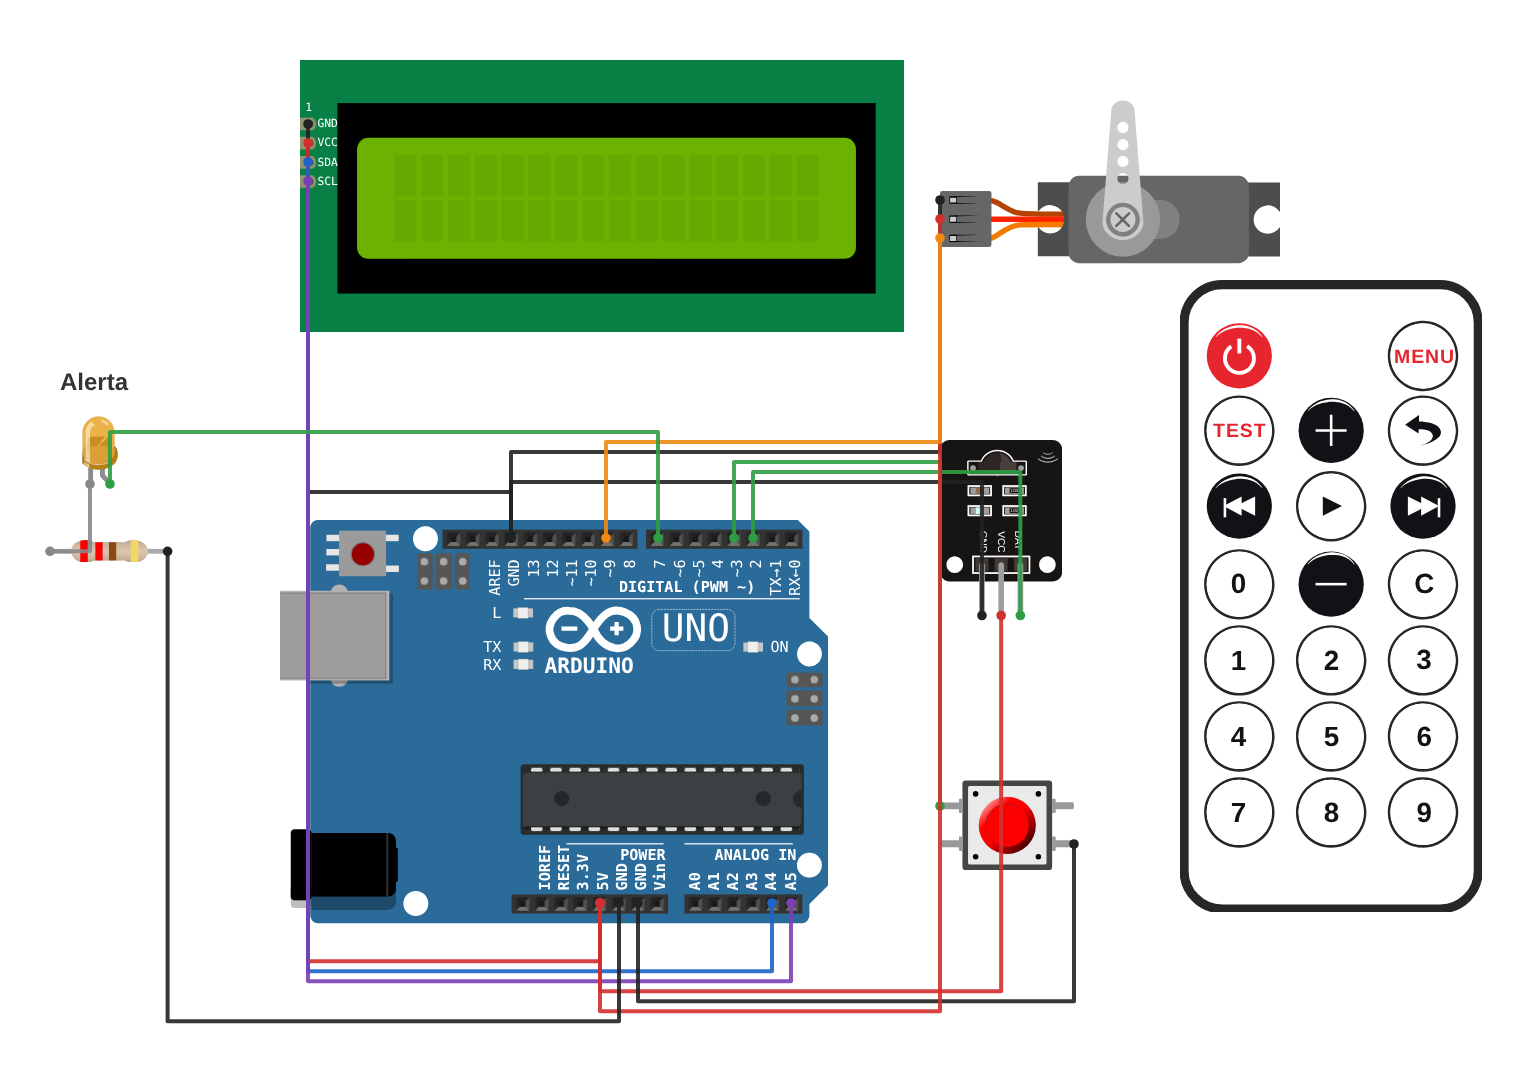
\includegraphics[width=.82\textwidth]{figuras/esquema-01.png}
\caption{Esquema do circuito da Automação 1, desenhado a partir do \texttt{diagram.json} com as peças do Wokwi}\label{fig:esq1}
\end{figure}

\paragraph{Funcionamento.} O portão é modelado como uma máquina de cinco estados (Tabela~\ref{tab:est1}). O servo anda um grau a cada 40 ms, cerca de 3,6 s de curso, o que imita a partida suave de um motor de portão. O fechamento automático acontece 15 s depois da abertura (2 minutos na prática), mas só se a barreira estiver livre. A recepção infravermelha usa a biblioteca IRremote, que ocupa o \emph{Timer2}; por isso o aviso é visual, e não sonoro, já que a função \texttt{tone()} disputaria o mesmo temporizador. A Tabela~\ref{tab:est1} resume as transições.

\begin{table}[ht]
\centering
\caption{Transições da Automação 1}\label{tab:est1}
\footnotesize
\begin{tabularx}{\textwidth}{lXlX}
\toprule
Estado & Evento & Próximo estado & Ação \\
\midrule
Fechado & PLAY ou + & Abrindo & Liga o pisca-alerta \\
Abrindo & chegou a 90$^\circ$ & Aberto & Inicia a contagem de 15 s \\
Aberto & 15 s sem obstáculo, PLAY ou $-$ & Fechando & Liga o pisca-alerta \\
Fechando & obstáculo na barreira & Abrindo & Reverte o movimento \\
Fechando & chegou a 0$^\circ$ & Fechado & Desliga o pisca-alerta \\
Abrindo/Fechando & POWER & Parado & Congela a posição \\
Parado & +, $-$ ou PLAY & Abrindo/Fechando & Retoma o movimento \\
\bottomrule
\end{tabularx}
\end{table}

\paragraph{Validação.} A Tabela~\ref{tab:val1} traz o roteiro de validação: cada estímulo aplicado e a resposta esperada, todos conferidos nos testes de lógica.

\begin{table}[ht]
\centering
\caption{Roteiro de validação da Automação 1}\label{tab:val1}
\footnotesize
\begin{tabularx}{\textwidth}{cXXc}
\toprule
Passo & Estímulo & Resposta & Situação \\
\midrule
1 & Tecla PLAY com o portão fechado & Servo sobe devagar, LED pisca, LCD ``ABRINDO'' & OK \\
2 & Aguardar o fim do curso & Servo em 90$^\circ$, LCD ``ABERTO'' e ``100\%'', LED apagado & OK \\
3 & Aguardar 15 s & Fecha sozinho & OK \\
4 & Apertar a barreira durante o fechamento & Reverte e reabre & OK \\
5 & Manter a barreira apertada com o portão aberto & Não fecha sozinho & OK \\
6 & Tecla $-$ e, no meio do curso, POWER & Portão para na posição atual & OK \\
7 & Tecla $-$ de novo & Termina de fechar & OK \\
8 & Tecla numérica (1) & Ignorada & OK \\
\bottomrule
\end{tabularx}
\end{table}

\subsection{Automação 2: Alarme residencial com tempos de saída e entrada}\label{sub:a2}

\paragraph{Descrição do problema.} Um alarme que dispara no instante em que a porta abre não permite que o próprio morador entre e o desarme; um alarme sem tempo de saída dispara quando ele sai de casa. Esta automação reproduz o comportamento das centrais comerciais: tempo de saída depois de armar, tempo de entrada para desarmar e disparo imediato para movimento dentro de casa.

\paragraph{Hardware.} Os componentes estão na Tabela~\ref{tab:hw2}. Ligações: Porta em D2; PIR em D3; botão em D4 (\emph{pull-up}); sirene em D8; LEDs em D9, D10 e D11; LCD em A4/A5. Projeto: pasta \pasta{02-alarme-residencial}.

\begin{table}[ht]
\centering
\caption{Hardware da Automação 2}\label{tab:hw2}
\footnotesize
\begin{tabularx}{\textwidth}{lX}
\toprule
Componente & Função \\
\midrule
Chave deslizante & Sensor magnético da porta (aberta/fechada) \\
Sensor PIR & Detecta presença na sala \\
Botão de comando & Toque curto arma; segurar 2 s desarma \\
Buzzer & Sirene e bipes de contagem \\
LEDs verde, amarelo e vermelho + resistores & Desarmado, contagem e armado/disparado \\
LCD 16x2 I2C & Situação e contagem regressiva \\
\bottomrule
\end{tabularx}
\end{table}

\begin{figure}[ht]
\centering
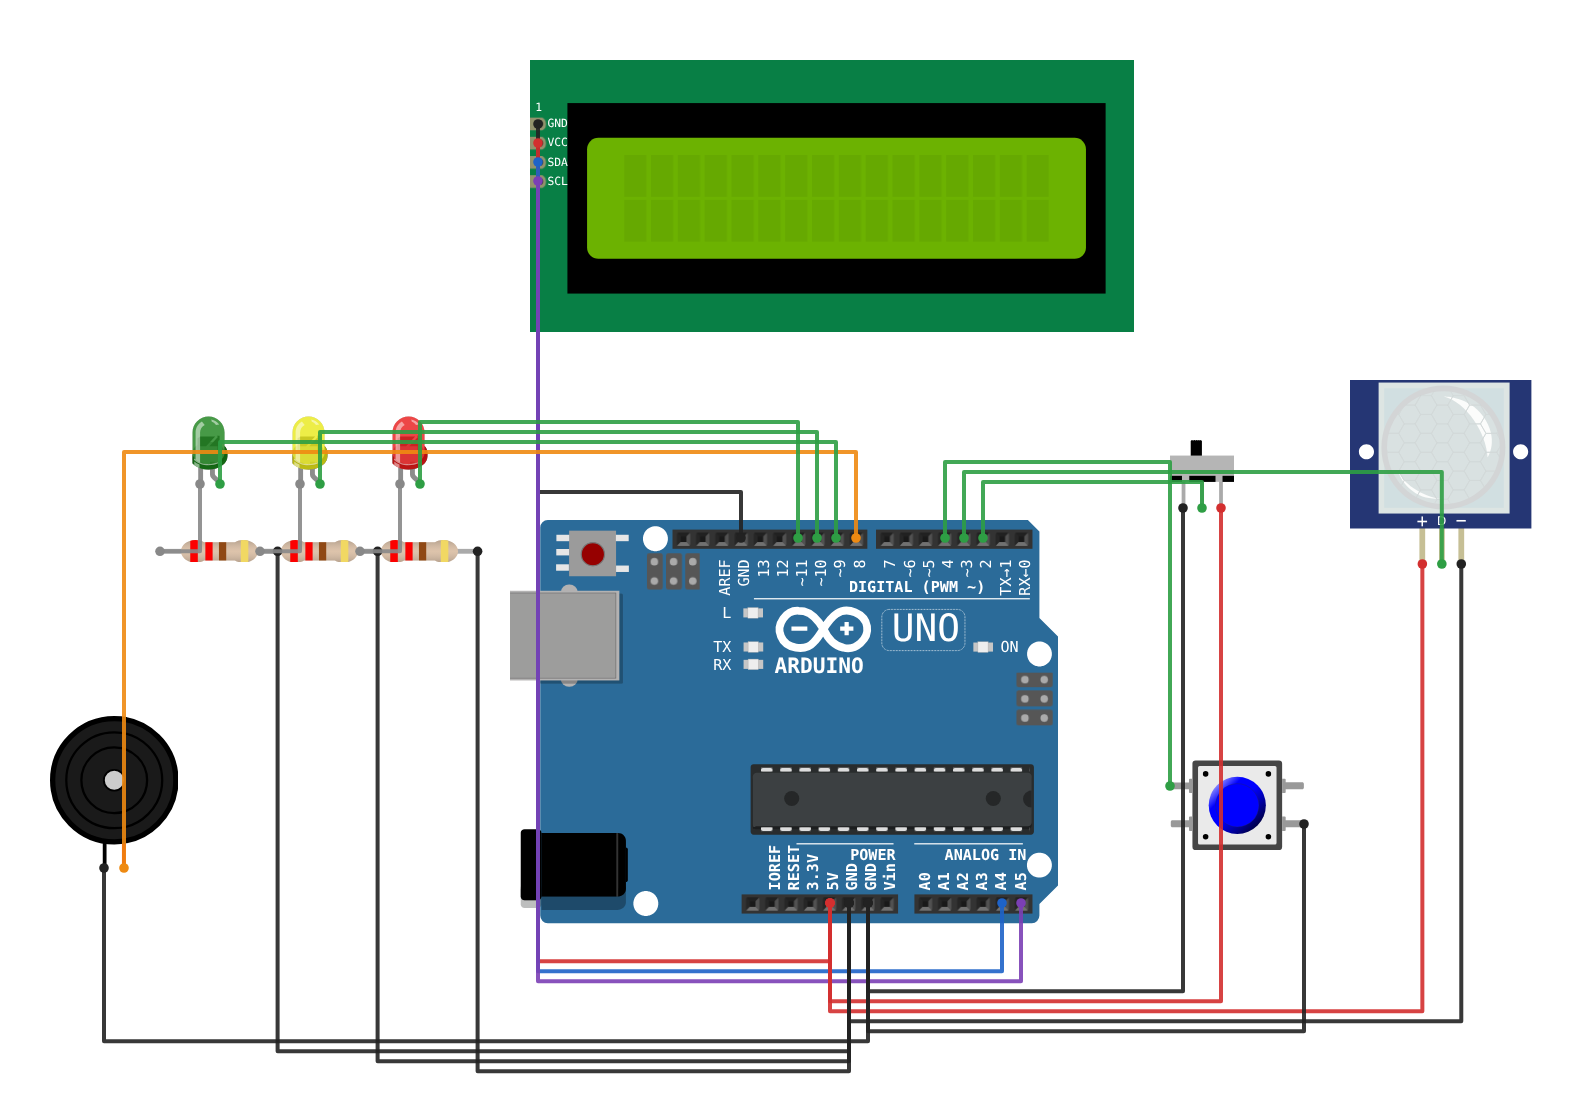
\includegraphics[width=.82\textwidth]{figuras/esquema-02.png}
\caption{Esquema do circuito da Automação 2, desenhado a partir do \texttt{diagram.json} com as peças do Wokwi}\label{fig:esq2}
\end{figure}

\paragraph{Funcionamento.} O botão único distingue toque curto e toque longo: o toque curto é reconhecido quando o botão é solto antes de 2 s, e o longo, quando passa de 2 s apertado. Desarmar exige o toque longo, o que evita que um esbarrão desligue o alarme. A sirene alterna dois tons e para sozinha depois de 30 s, para não perturbar a vizinhança, mas o LED vermelho continua piscando até alguém desarmar. Os tempos estão em 10 s, valor comum nas centrais reais. A Tabela~\ref{tab:est2} resume as transições.

\begin{table}[ht]
\centering
\caption{Transições da Automação 2}\label{tab:est2}
\footnotesize
\begin{tabularx}{\textwidth}{lXlX}
\toprule
Estado & Evento & Próximo estado & Ação \\
\midrule
Desarmado & toque curto & Saída & Bipe por segundo, LED amarelo piscando \\
Saída & 10 s com a porta fechada & Armado & LED vermelho fixo \\
Saída & 10 s com a porta aberta & Disparado & Sirene (``Porta aberta'') \\
Armado & porta abriu & Entrada & Bipe rápido por segundo \\
Armado & movimento no PIR & Disparado & Sirene (``Presença interna'') \\
Entrada & 10 s sem desarmar & Disparado & Sirene (``Invasão porta'') \\
qualquer um & segurar 2 s & Desarmado & Desliga a sirene, LED verde \\
\bottomrule
\end{tabularx}
\end{table}

\paragraph{Validação.} A Tabela~\ref{tab:val2} traz o roteiro de validação: cada estímulo aplicado e a resposta esperada, todos conferidos nos testes de lógica.

\begin{table}[ht]
\centering
\caption{Roteiro de validação da Automação 2}\label{tab:val2}
\footnotesize
\begin{tabularx}{\textwidth}{cXXc}
\toprule
Passo & Estímulo & Resposta & Situação \\
\midrule
1 & Toque curto no botão & ``Saia e feche'' com contagem de 10 s & OK \\
2 & Aguardar 10 s com a porta fechada & ``ARMADO'', LED vermelho & OK \\
3 & Abrir a porta (chave) & Contagem de entrada com bipe rápido & OK \\
4 & Segurar o botão 2 s & ``DESARMADO'', LED verde & OK \\
5 & Armar, abrir a porta e não desarmar & Disparo ``Invasao porta'', sirene & OK \\
6 & Aguardar 30 s & Sirene para, LED vermelho segue piscando & OK \\
7 & Armar e simular movimento no PIR & Disparo imediato ``Presenca interna'' & OK \\
8 & Armar com a porta aberta & Dispara ao fim do tempo de saída & OK \\
9 & Toque curto durante o disparo & Não desarma & OK \\
\bottomrule
\end{tabularx}
\end{table}

\subsection{Automação 3: Luz do corredor com presença e vigília}\label{sub:a3}

\paragraph{Descrição do problema.} À noite, quem levanta para ir à cozinha ou ao banheiro procura o interruptor no escuro; deixar a luz acesa a noite toda, por outro lado, gasta energia e atrapalha o sono. A automação mantém uma luz fraca de vigília no corredor e acende a lâmpada por completo quando alguém passa, apagando devagar depois. De dia, a lâmpada fica desligada.

\paragraph{Hardware.} Os componentes estão na Tabela~\ref{tab:hw3}. Ligações: PIR em D2; LDR (saída AO) em A0; lâmpada em D9 (PWM). Projeto: pasta \pasta{03-luz-corredor}.

\begin{table}[ht]
\centering
\caption{Hardware da Automação 3}\label{tab:hw3}
\footnotesize
\begin{tabularx}{\textwidth}{lX}
\toprule
Componente & Função \\
\midrule
Sensor PIR & Detecta a passagem de pessoas \\
Módulo LDR & Diferencia dia e noite \\
LED branco + resistor 220 $\Omega$ & Lâmpada dimerizável (PWM) \\
\bottomrule
\end{tabularx}
\end{table}

\begin{figure}[ht]
\centering
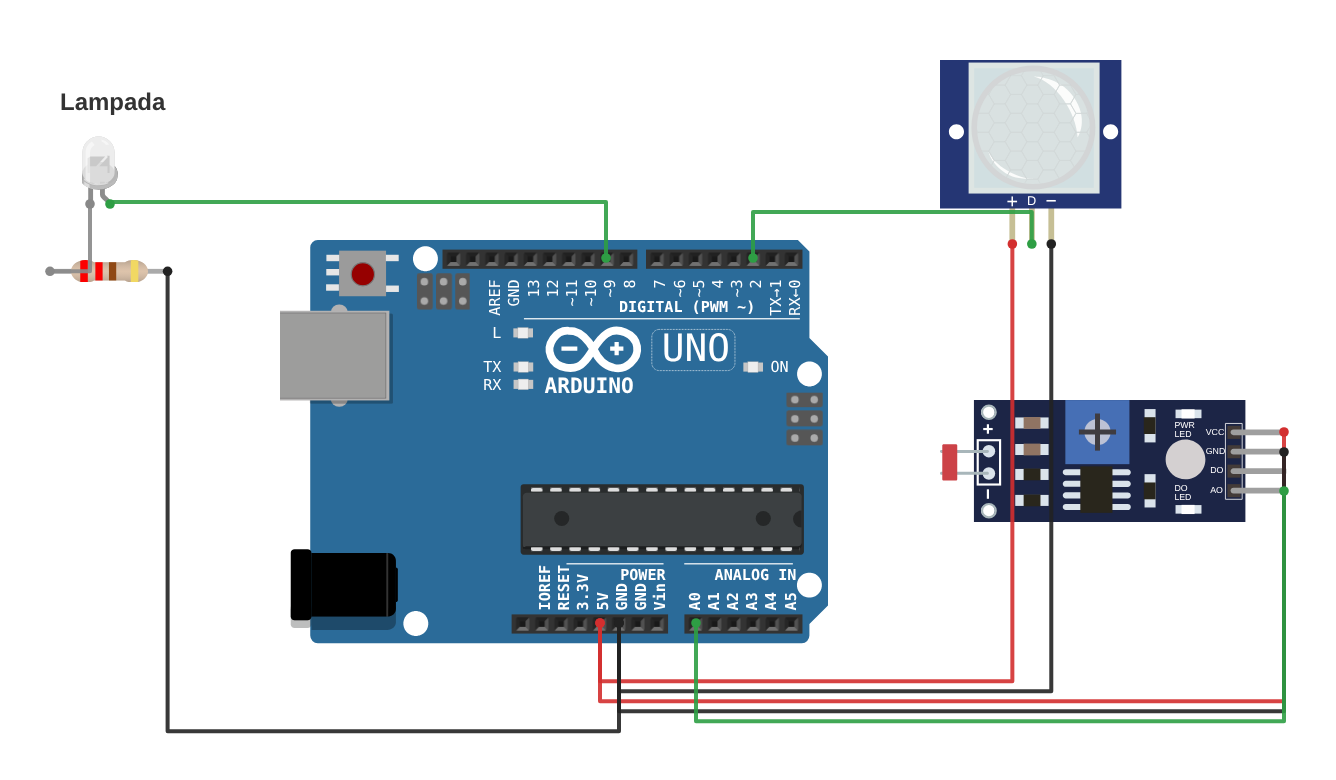
\includegraphics[width=.82\textwidth]{figuras/esquema-03.png}
\caption{Esquema do circuito da Automação 3, desenhado a partir do \texttt{diagram.json} com as peças do Wokwi}\label{fig:esq3}
\end{figure}

\paragraph{Funcionamento.} Dia e noite são decididos com histerese sobre a leitura do LDR: acima de 600 (cerca de 60 lux) passa a ser noite e só abaixo de 520 (cerca de 100 lux) volta a ser dia, o que evita que a lâmpada pisque ao entardecer. O brilho desejado é 0\% de dia, 10\% à noite sem presença e 100\% nos 20 s seguintes ao último movimento. O brilho real segue o desejado em rampa, um degrau de PWM a cada 8 ms, de modo que a luz acende e apaga suavemente, sem ofuscar quem acabou de acordar. O algoritmo abaixo resume a decisão.

\begin{lstlisting}[style=algo]
a cada ciclo:
  leitura <- LDR
  se é dia e leitura > 600: noite <- verdadeiro
  se é noite e leitura < 520: noite <- falso
  se PIR ativo: últimoMovimento <- agora
  se não noite:                          alvo <- 0
  senão se agora - últimoMovimento < 20 s: alvo <- 255
  senão:                                 alvo <- 26 (vigília)
  a cada 8 ms: brilho <- brilho +1 ou -1 em direção ao alvo
\end{lstlisting}

\paragraph{Validação.} A Tabela~\ref{tab:val3} traz o roteiro de validação: cada estímulo aplicado e a resposta esperada, todos conferidos nos testes de lógica.

\begin{table}[ht]
\centering
\caption{Roteiro de validação da Automação 3}\label{tab:val3}
\footnotesize
\begin{tabularx}{\textwidth}{cXXc}
\toprule
Passo & Estímulo & Resposta & Situação \\
\midrule
1 & LDR claro (dia) & Lâmpada apagada & OK \\
2 & Movimento de dia & Continua apagada & OK \\
3 & LDR escuro (noite), sem movimento & Luz de vigília em 10\% & OK \\
4 & Leitura entre os dois limiares & Não muda de dia para noite (histerese) & OK \\
5 & Movimento à noite & Acende em rampa até 100\% & OK \\
6 & Aguardar 17 s parado & Continua acesa & OK \\
7 & Completar 20 s sem movimento & Volta suavemente para 10\% & OK \\
8 & LDR claro de novo & Apaga & OK \\
\bottomrule
\end{tabularx}
\end{table}

\subsection{Automação 4: Cortina motorizada do quarto}\label{sub:a4}

\paragraph{Descrição do problema.} Em quartos voltados para o poente, o sol direto da tarde aquece o ambiente e ofusca quem está no computador; à noite, a cortina aberta expõe a casa. A automação abre a cortina ao amanhecer, fecha ao anoitecer e fecha pela metade quando o sol bate direto, com um modo manual para quando o morador prefere decidir.

\paragraph{Hardware.} Os componentes estão na Tabela~\ref{tab:hw4}. Ligações: Abrir em D2 e Fechar em D3 (\emph{pull-up}); chave de modo em D4; servo em D6; LDR em A0; LCD em A4/A5. Projeto: pasta \pasta{04-cortina-automatica}.

\begin{table}[ht]
\centering
\caption{Hardware da Automação 4}\label{tab:hw4}
\footnotesize
\begin{tabularx}{\textwidth}{lX}
\toprule
Componente & Função \\
\midrule
Módulo LDR & Mede a luz que chega à janela \\
Chave deslizante & Seleciona modo automático ou manual \\
Botões ``Abrir'' e ``Fechar'' & Ajuste manual em passos de 25\% \\
Servo motor & Movimenta a cortina (0$^\circ$ fechada, 180$^\circ$ aberta) \\
LCD 16x2 I2C & Abertura, modo e luz medida \\
\bottomrule
\end{tabularx}
\end{table}

\begin{figure}[ht]
\centering
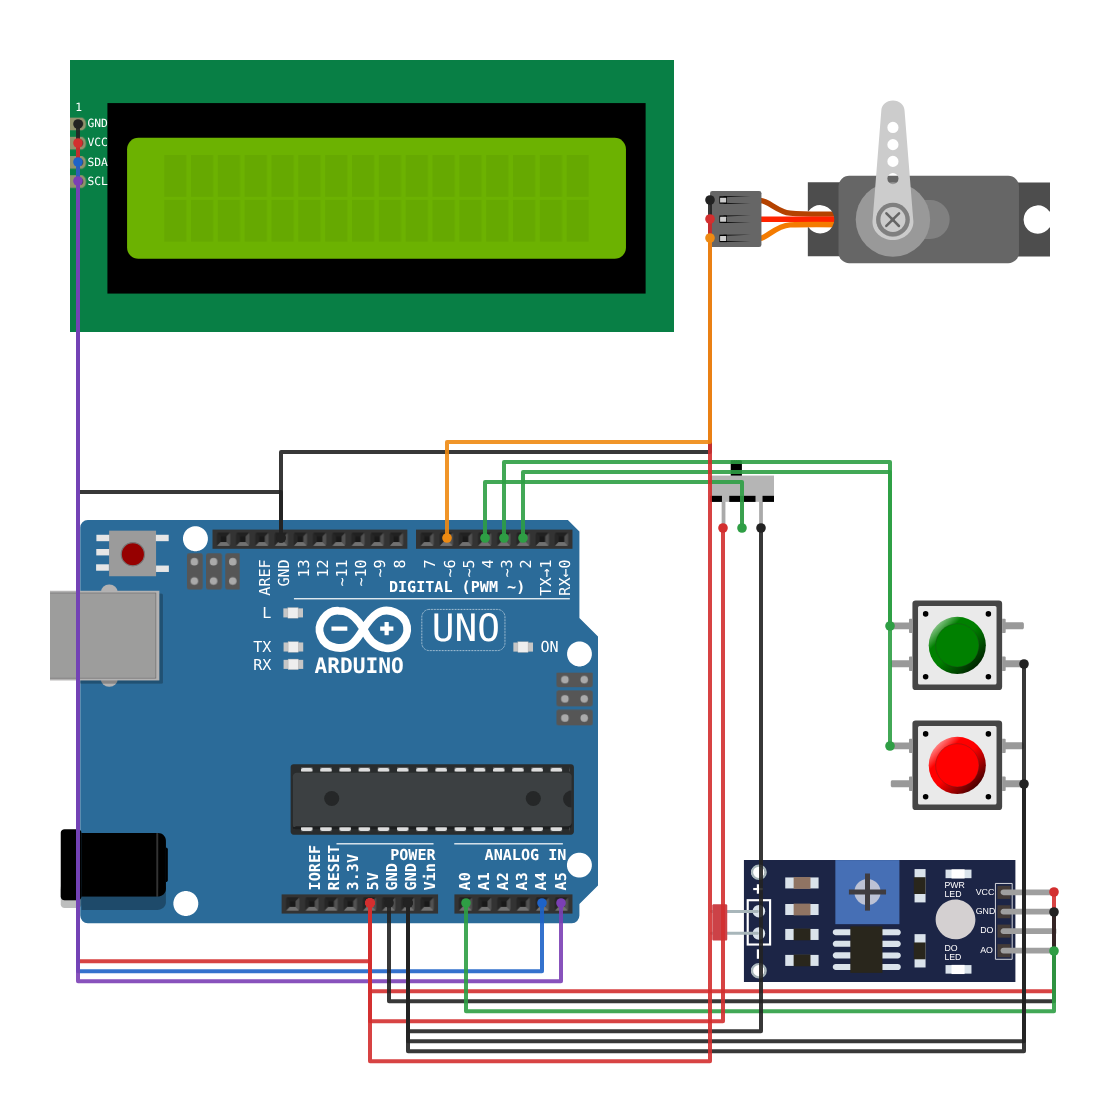
\includegraphics[width=.82\textwidth]{figuras/esquema-04.png}
\caption{Esquema do circuito da Automação 4, desenhado a partir do \texttt{diagram.json} com as peças do Wokwi}\label{fig:esq4}
\end{figure}

\paragraph{Funcionamento.} A leitura do LDR é convertida em lux pela curva do componente. No modo automático, a decisão depende da posição atual (Tabela~\ref{tab:est4}), o que cria histerese: a cortina abre acima de 50 lux mas só fecha abaixo de 10 lux; vai para 50\% acima de 20\,000 lux e só volta a abrir abaixo de 12\,000 lux. Assim, uma nuvem passando não faz a cortina subir e descer. O servo anda 1\% a cada 15 ms. Os botões são lidos sempre, mas só têm efeito no modo manual. A Tabela~\ref{tab:est4} resume as transições.

\begin{table}[ht]
\centering
\caption{Transições da Automação 4}\label{tab:est4}
\footnotesize
\begin{tabularx}{\textwidth}{lXlX}
\toprule
Estado & Evento & Próximo estado & Ação \\
\midrule
Fechada (0\%) & luz > 50 lux & Aberta (100\%) & Abre devagar \\
Aberta (100\%) & luz < 10 lux & Fechada (0\%) & Fecha devagar \\
Aberta (100\%) & luz > 20\,000 lux & Meia (50\%) & Protege do sol direto \\
Meia (50\%) & luz < 12\,000 lux & Aberta (100\%) & Reabre \\
Meia (50\%) & luz < 10 lux & Fechada (0\%) & Fecha \\
\bottomrule
\end{tabularx}
\end{table}

\paragraph{Validação.} A Tabela~\ref{tab:val4} traz o roteiro de validação: cada estímulo aplicado e a resposta esperada, todos conferidos nos testes de lógica.

\begin{table}[ht]
\centering
\caption{Roteiro de validação da Automação 4}\label{tab:val4}
\footnotesize
\begin{tabularx}{\textwidth}{cXXc}
\toprule
Passo & Estímulo & Resposta & Situação \\
\midrule
1 & Modo auto, LDR a 2 lux & Cortina fechada & OK \\
2 & LDR a 30 lux & Continua fechada (histerese) & OK \\
3 & LDR a 400 lux & Abre até 100\% (servo a 180$^\circ$) & OK \\
4 & LDR a 50\,000 lux & Vai para 50\% & OK \\
5 & LDR a 15\,000 lux & Mantém 50\% & OK \\
6 & LDR a 5\,000 lux & Volta a 100\% & OK \\
7 & LDR a 5 lux & Fecha & OK \\
8 & Modo manual, dois toques em Abrir & 50\%, sem reagir à luz & OK \\
9 & Um toque em Fechar & 25\%; LCD indica MANUAL & OK \\
\bottomrule
\end{tabularx}
\end{table}

\subsection{Automação 5: Irrigação do jardim por umidade do solo}\label{sub:a5}

\paragraph{Descrição do problema.} Regar o jardim em horário fixo desperdiça água em dias úmidos ou chuvosos, e regar de uma vez só encharca a superfície enquanto a água escorre sem infiltrar. A automação rega apenas quando o solo está seco e não chove, em ciclos curtos de rega e pausa, e para com aviso se a umidade não sobe, o que indica vazamento ou sensor com defeito.

\paragraph{Hardware.} Os componentes estão na Tabela~\ref{tab:hw5}. Ligações: Botão em D2 (\emph{pull-up}); chave de chuva em D4; relé em D7; potenciômetro em A0; LCD em A4/A5. Projeto: pasta \pasta{05-irrigacao-jardim}.

\begin{table}[ht]
\centering
\caption{Hardware da Automação 5}\label{tab:hw5}
\footnotesize
\begin{tabularx}{\textwidth}{lX}
\toprule
Componente & Função \\
\midrule
Potenciômetro & Representa o sensor de umidade do solo (0 a 100\%) \\
Chave deslizante & Representa o sensor de chuva \\
Botão ``Regar agora'' & Rega manual de 5 s e reconhecimento de falha \\
Módulo relé + LED azul & Válvula solenoide da rede de gotejamento \\
LCD 16x2 I2C & Umidade, chuva e etapa \\
\bottomrule
\end{tabularx}
\end{table}

\begin{figure}[ht]
\centering
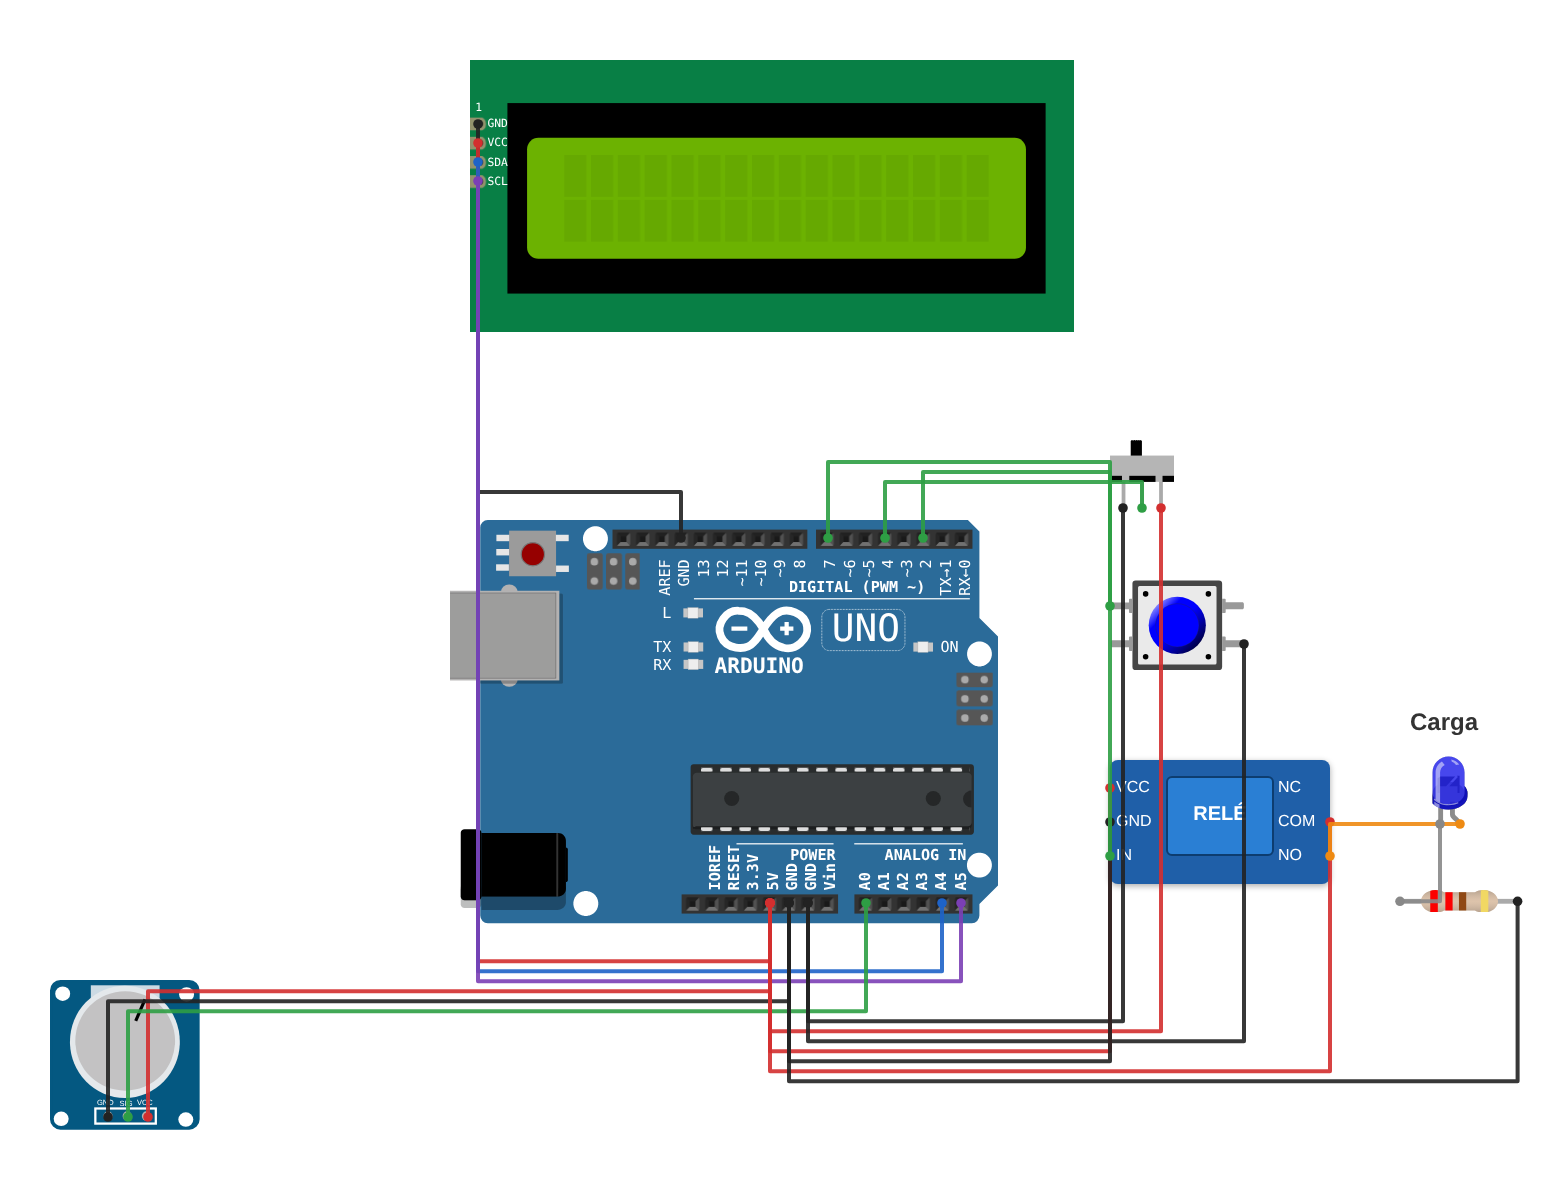
\includegraphics[width=.82\textwidth]{figuras/esquema-05.png}
\caption{Esquema do circuito da Automação 5, desenhado a partir do \texttt{diagram.json} com as peças do Wokwi}\label{fig:esq5}
\end{figure}

\paragraph{Funcionamento.} O Wokwi não tem sensor de umidade do solo; o potenciômetro gera a mesma faixa de tensão de um sensor capacitivo e permite testar todos os casos. A rega começa abaixo de 30\% e termina ao chegar a 60\%. Cada ciclo tem 8 s de rega e 10 s de infiltração (5 e 20 minutos na prática). Depois de 4 ciclos sem atingir 60\%, o sistema entra em falha e fecha a válvula. A chuva cancela a rega em qualquer etapa. A Tabela~\ref{tab:est5} resume as transições.

\begin{table}[ht]
\centering
\caption{Transições da Automação 5}\label{tab:est5}
\footnotesize
\begin{tabularx}{\textwidth}{lXlX}
\toprule
Estado & Evento & Próximo estado & Ação \\
\midrule
Aguardando & solo < 30\% e sem chuva & Regando (ciclo 1) & Abre a válvula \\
Aguardando & botão e sem chuva & Rega manual & Abre a válvula por 5 s \\
Regando & passaram 8 s & Infiltrando & Fecha a válvula \\
Regando ou Infiltrando & solo $\geq$ 60\% & Aguardando & Fecha a válvula \\
Infiltrando & 10 s e ciclo < 4 & Regando (ciclo + 1) & Abre a válvula \\
Infiltrando & 10 s e ciclo = 4 & Falha & Válvula fechada, aviso no LCD \\
qualquer rega & chuva & Aguardando & Fecha a válvula \\
Falha & botão & Aguardando & Reconhece o aviso \\
\bottomrule
\end{tabularx}
\end{table}

\paragraph{Validação.} A Tabela~\ref{tab:val5} traz o roteiro de validação: cada estímulo aplicado e a resposta esperada, todos conferidos nos testes de lógica.

\begin{table}[ht]
\centering
\caption{Roteiro de validação da Automação 5}\label{tab:val5}
\footnotesize
\begin{tabularx}{\textwidth}{cXXc}
\toprule
Passo & Estímulo & Resposta & Situação \\
\midrule
1 & Solo em 50\% & Não rega & OK \\
2 & Solo em 20\% & Relé liga (LED azul aceso) & OK \\
3 & Aguardar 8 s & ``Infiltrando'', válvula fechada & OK \\
4 & Aguardar 10 s com o solo seco & Segundo ciclo de rega & OK \\
5 & Subir o solo para 65\% & Para e volta a ``Aguardando'' & OK \\
6 & Solo seco e ligar a chave de chuva & Rega cancelada na hora & OK \\
7 & Botão com chuva & Não rega & OK \\
8 & Desligar a chuva e manter o solo seco por 4 ciclos & ``FALHA: verificar'' & OK \\
9 & Botão na falha; botão de novo & Reconhece; depois rega manual de 5 s & OK \\
\bottomrule
\end{tabularx}
\end{table}

\subsection{Automação 6: Ventilador de teto com velocidade automática}\label{sub:a6}

\paragraph{Descrição do problema.} Ventiladores de teto costumam ficar na mesma velocidade a noite toda: rápido demais de madrugada, quando esfria, ou fraco demais no começo da noite. A automação escolhe a velocidade pela sensação térmica do ambiente e mostra a velocidade num display, mantendo o comando manual pelo botão.

\paragraph{Hardware.} Os componentes estão na Tabela~\ref{tab:hw6}. Ligações: DHT22 em D2; botão em D3 (\emph{pull-up}); segmentos a--g e ponto em D4, D5, D6, D7, D8, D10, D11 e D12; comum do display no GND; motor em D9 (PWM). Projeto: pasta \pasta{06-ventilador-teto}.

\begin{table}[ht]
\centering
\caption{Hardware da Automação 6}\label{tab:hw6}
\footnotesize
\begin{tabularx}{\textwidth}{lX}
\toprule
Componente & Função \\
\midrule
Sensor DHT22 & Temperatura e umidade do quarto \\
Botão de modo & Auto, 1, 2, 3 e Desligado, em sequência \\
Display de 7 segmentos (catodo comum) & Velocidade atual; ponto aceso no modo automático \\
LED azul + resistor 220 $\Omega$ & Motor do ventilador (brilho proporcional à velocidade) \\
\bottomrule
\end{tabularx}
\end{table}

\begin{figure}[ht]
\centering
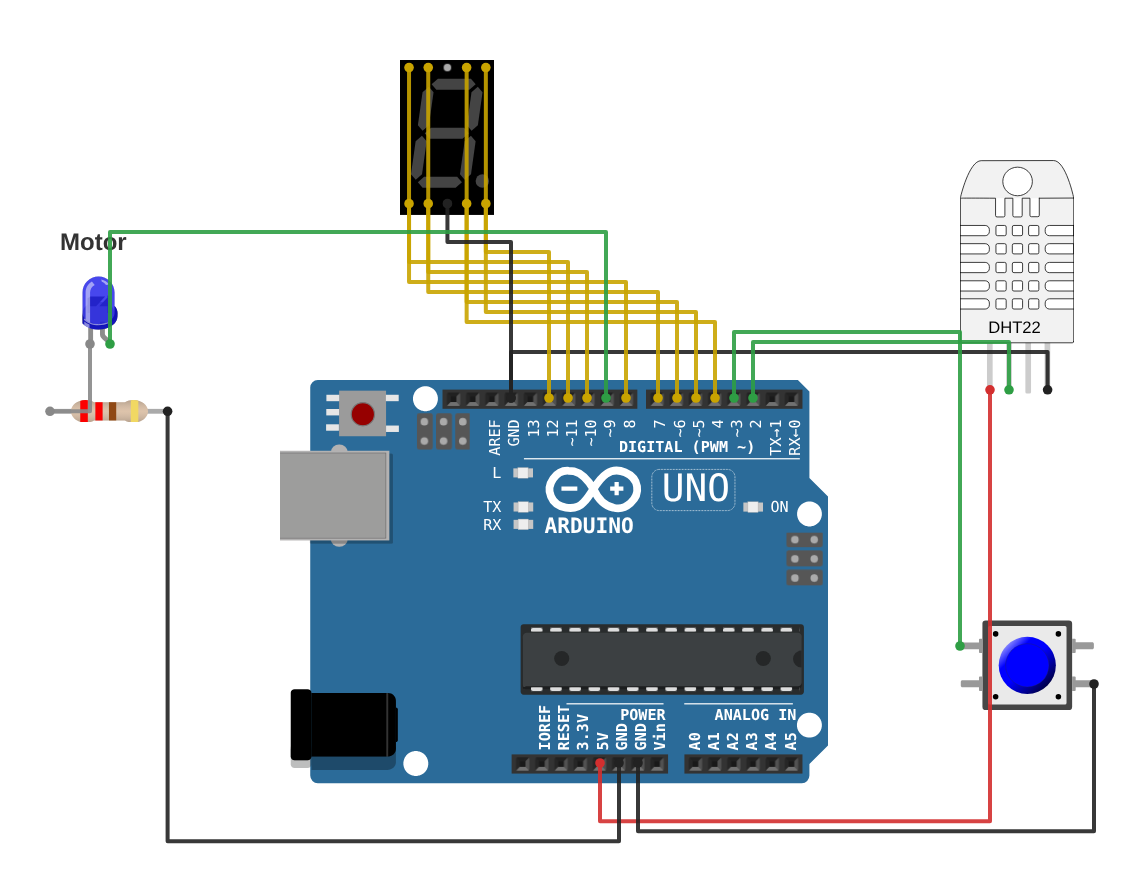
\includegraphics[width=.82\textwidth]{figuras/esquema-06.png}
\caption{Esquema do circuito da Automação 6, desenhado a partir do \texttt{diagram.json} com as peças do Wokwi}\label{fig:esq6}
\end{figure}

\paragraph{Funcionamento.} A sensação térmica é estimada somando 0,5 $^\circ$C a cada 10\% de umidade acima de 60\%, uma simplificação do índice de calor que reflete a menor evaporação do suor em ar úmido. As velocidades mudam nos limites de 24; 26,5 e 29 $^\circ$C, e cada degrau só é desfeito meio grau abaixo do limite (histerese), para o ventilador não ficar trocando de velocidade. O display é acionado diretamente pelos pinos, sem biblioteca, a partir de uma tabela de bits com o desenho de cada dígito. Sem leitura válida do sensor, o modo automático mantém a velocidade 1 por segurança. O algoritmo abaixo resume a decisão.

\begin{lstlisting}[style=algo]
a cada 2 s: T, UR <- DHT22
  sensação <- T + max(0, UR - 60) * 0,05
se botão apertado: modo <- próximo (Auto, 1, 2, 3, Desligado)
se modo = Auto:
  v <- velocidade atual
  enquanto v < 3 e sensação >= limite[v]:          v <- v + 1
  enquanto v > 0 e sensação < limite[v-1] - 0,5:   v <- v - 1
senão: v <- velocidade fixa do modo (0 no Desligado)
PWM do motor <- {0, 90, 170, 255}[v]
display <- dígito v; ponto aceso se modo = Auto
\end{lstlisting}

\paragraph{Validação.} A Tabela~\ref{tab:val6} traz o roteiro de validação: cada estímulo aplicado e a resposta esperada, todos conferidos nos testes de lógica.

\begin{table}[ht]
\centering
\caption{Roteiro de validação da Automação 6}\label{tab:val6}
\footnotesize
\begin{tabularx}{\textwidth}{cXXc}
\toprule
Passo & Estímulo & Resposta & Situação \\
\midrule
1 & 22 $^\circ$C e 50\% & Display ``0.'' (ponto = automático), motor parado & OK \\
2 & 25 $^\circ$C & Velocidade 1 & OK \\
3 & 27 $^\circ$C & Velocidade 2 & OK \\
4 & 30 $^\circ$C & Velocidade 3, motor no máximo & OK \\
5 & 28,7 $^\circ$C & Mantém 3 (histerese) & OK \\
6 & 28,4 $^\circ$C & Cai para 2 & OK \\
7 & 25,5 $^\circ$C com 90\% de umidade & Velocidade 2 (sensação de 27 $^\circ$C) & OK \\
8 & Botão (modo manual 1) & Display ``1'' sem ponto & OK \\
9 & Mais dois toques; mais um & Velocidade 3; depois desligado & OK \\
10 & Mais um toque & Volta ao automático & OK \\
\bottomrule
\end{tabularx}
\end{table}

\subsection{Automação 7: Comedouro automático do pet com balança}\label{sub:a7}

\paragraph{Descrição do problema.} Comedouros por tempo liberam ração mesmo que o pote ainda esteja cheio, o que leva a excesso e desperdício, e não percebem quando o reservatório acaba. Este comedouro pesa o pote: serve só o que falta para a porção, deixa de servir se o animal não comeu a refeição anterior e avisa quando a ração não cai.

\paragraph{Hardware.} Os componentes estão na Tabela~\ref{tab:hw7}. Ligações: HX711: DT em A1 e SCK em A0; botão em D2 (\emph{pull-up}); servo em D6; buzzer em D8; LED em D9; LCD em A4/A5. Projeto: pasta \pasta{07-comedouro-pet}.

\begin{table}[ht]
\centering
\caption{Hardware da Automação 7}\label{tab:hw7}
\footnotesize
\begin{tabularx}{\textwidth}{lX}
\toprule
Componente & Função \\
\midrule
Célula de carga 5 kg + módulo HX711 & Peso do pote de ração \\
Botão ``Servir agora'' & Refeição extra e confirmação de reabastecimento \\
Servo motor & Comporta do reservatório \\
Buzzer & Sinal de refeição servida e alerta \\
LED vermelho + resistor 220 $\Omega$ & Reservatório vazio \\
LCD 16x2 I2C & Peso, situação e tempo para a próxima refeição \\
\bottomrule
\end{tabularx}
\end{table}

\begin{figure}[ht]
\centering
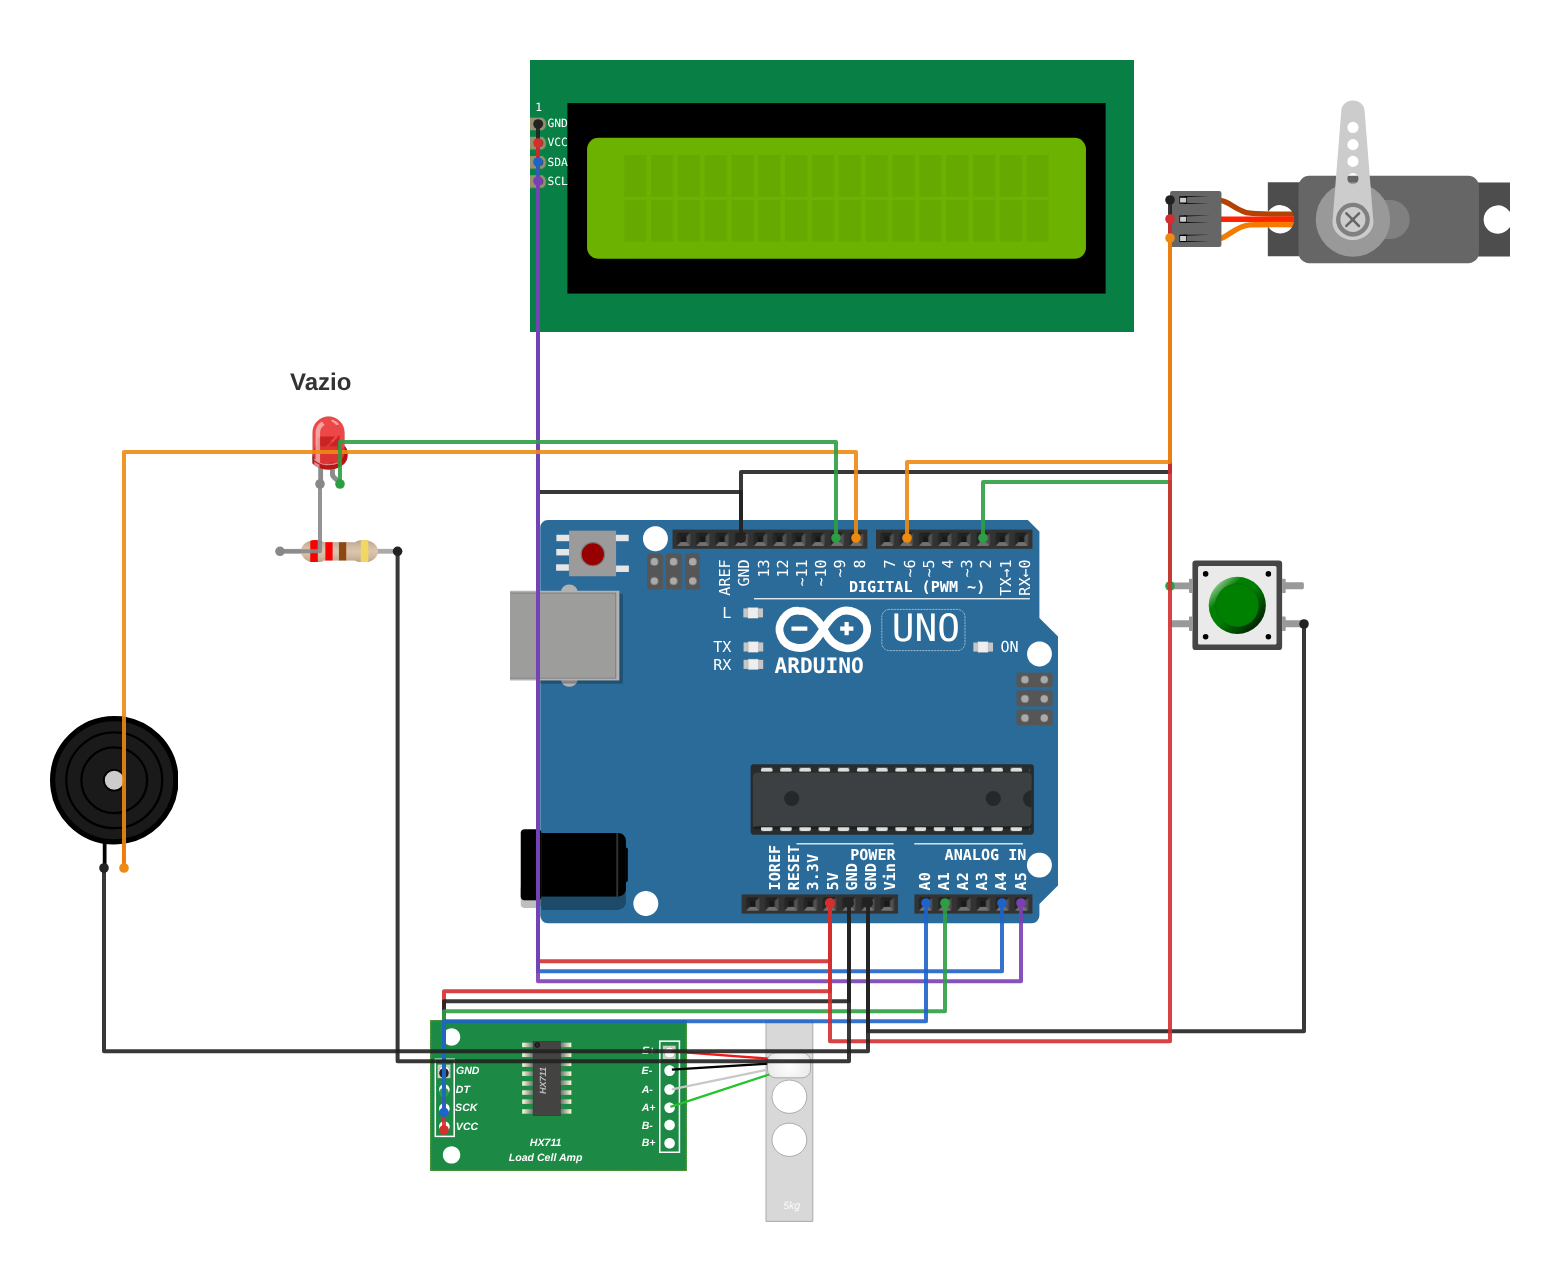
\includegraphics[width=.82\textwidth]{figuras/esquema-07.png}
\caption{Esquema do circuito da Automação 7, desenhado a partir do \texttt{diagram.json} com as peças do Wokwi}\label{fig:esq7}
\end{figure}

\paragraph{Funcionamento.} No Wokwi, a célula de 5 kg entrega leituras brutas de 0 a 2100; com a escala de 0,42 a biblioteca HX711 devolve o peso em gramas. A cada 30 s (8 horas na prática) ou pelo botão, o sistema verifica o pote: com 60 g ou mais, não serve; com menos, abre a comporta até o peso atingir 100 g. Se a porção não é atingida em 8 s, conclui que o reservatório está vazio, fecha a comporta e passa a bipar a cada 3 s. O botão, depois do reabastecimento, faz uma nova tentativa. A Tabela~\ref{tab:est7} resume as transições.

\begin{table}[ht]
\centering
\caption{Transições da Automação 7}\label{tab:est7}
\footnotesize
\begin{tabularx}{\textwidth}{lXlX}
\toprule
Estado & Evento & Próximo estado & Ação \\
\midrule
Esperando & horário ou botão, pote < 60 g & Servindo & Abre a comporta \\
Esperando & horário ou botão, pote $\geq$ 60 g & Esperando & Não serve, bipe curto \\
Servindo & peso $\geq$ 100 g & Esperando & Fecha a comporta, bipe agudo \\
Servindo & 8 s sem atingir a porção & Vazio & Fecha a comporta, LED aceso \\
Vazio & a cada 3 s & Vazio & Bipe de alerta \\
Vazio & botão (reabastecido) & Servindo & Nova tentativa \\
\bottomrule
\end{tabularx}
\end{table}

\paragraph{Validação.} A Tabela~\ref{tab:val7} traz o roteiro de validação: cada estímulo aplicado e a resposta esperada, todos conferidos nos testes de lógica.

\begin{table}[ht]
\centering
\caption{Roteiro de validação da Automação 7}\label{tab:val7}
\footnotesize
\begin{tabularx}{\textwidth}{cXXc}
\toprule
Passo & Estímulo & Resposta & Situação \\
\midrule
1 & Pote com 20 g, apertar o botão & Comporta abre (servo a 70$^\circ$) & OK \\
2 & Subir o peso para 60 g & Continua servindo & OK \\
3 & Subir para 105 g & Fecha a comporta, bipe, contador de refeições & OK \\
4 & Botão com o pote cheio & Não serve & OK \\
5 & Pote com 10 g, aguardar 30 s & Serve sozinho no horário & OK \\
6 & Não aumentar o peso por 8 s & ``RACAO ACABOU!'', LED aceso, bipes & OK \\
7 & Botão (reabastecido) & Tenta servir de novo & OK \\
8 & Subir o peso para 120 g & Serve e apaga o aviso & OK \\
\bottomrule
\end{tabularx}
\end{table}

\subsection{Automação 8: Campainha com modo ``não perturbe''}\label{sub:a8}

\paragraph{Descrição do problema.} A campainha tradicional toca a qualquer hora, acorda um bebê ou interrompe uma reunião por vídeo, e não registra quem veio enquanto ninguém atendeu. A automação toca uma melodia curta, conta as visitas, ignora o toque insistente da mesma pessoa e, no modo ``não perturbe'', troca o som por um aviso luminoso e guarda as visitas perdidas.

\paragraph{Hardware.} Os componentes estão na Tabela~\ref{tab:hw8}. Ligações: Botão em D2 (\emph{pull-up}); chave em D4; buzzer em D8; LED em D9; LCD em A4/A5. Projeto: pasta \pasta{08-campainha}.

\begin{table}[ht]
\centering
\caption{Hardware da Automação 8}\label{tab:hw8}
\footnotesize
\begin{tabularx}{\textwidth}{lX}
\toprule
Componente & Função \\
\midrule
Botão da campainha & Acionado pelo visitante \\
Chave deslizante & Liga e desliga o modo ``não perturbe'' \\
Buzzer & Melodia de três notas \\
LED azul + resistor 220 $\Omega$ & Aviso luminoso \\
LCD 16x2 I2C & Visitas, avisos e visitas perdidas \\
\bottomrule
\end{tabularx}
\end{table}

\begin{figure}[ht]
\centering
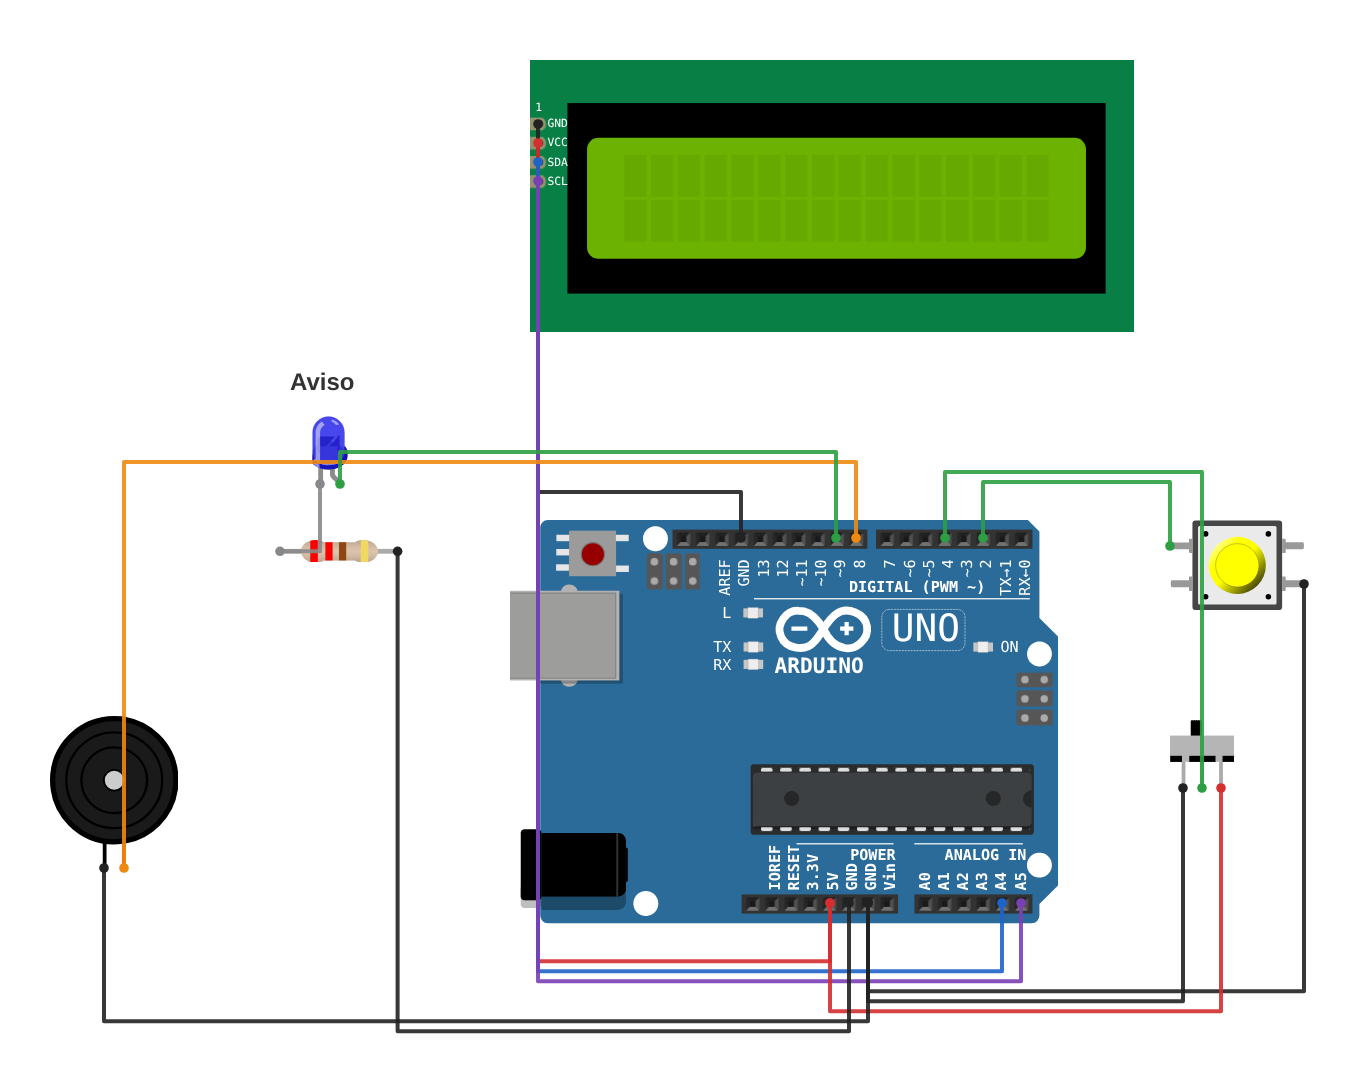
\includegraphics[width=.82\textwidth]{figuras/esquema-08.png}
\caption{Esquema do circuito da Automação 8, desenhado a partir do \texttt{diagram.json} com as peças do Wokwi}\label{fig:esq8}
\end{figure}

\paragraph{Funcionamento.} A melodia é tocada sem bloquear o programa: um vetor guarda frequência e duração de cada nota, e o laço principal avança para a nota seguinte quando o tempo da atual termina. Assim, o botão e a chave continuam sendo lidos durante a música. Toques em menos de 4 s após o anterior são tratados como a mesma visita. Quando o modo ``não perturbe'' é desligado, o LCD mostra quantas visitas ocorreram em silêncio. O algoritmo abaixo resume a decisão.

\begin{lstlisting}[style=algo]
se botão apertado:
  se o último toque foi há menos de 4 s: ignorar (mesma visita)
  senão:
    visitas <- visitas + 1; LED pisca por 5 s
    se não perturbe: perdidas <- perdidas + 1   (sem som)
    senão: iniciar melodia (nota 1)
se a nota atual terminou: tocar a próxima ou silenciar
se a chave mudou de "não perturbe" para normal e perdidas > 0:
  mostrar "N perdida(s)"; perdidas <- 0
\end{lstlisting}

\paragraph{Validação.} A Tabela~\ref{tab:val8} traz o roteiro de validação: cada estímulo aplicado e a resposta esperada, todos conferidos nos testes de lógica.

\begin{table}[ht]
\centering
\caption{Roteiro de validação da Automação 8}\label{tab:val8}
\footnotesize
\begin{tabularx}{\textwidth}{cXXc}
\toprule
Passo & Estímulo & Resposta & Situação \\
\midrule
1 & Apertar a campainha & Melodia de 3 notas, ``Ding-dong!'', visita 1 & OK \\
2 & Apertar de novo logo em seguida & Ignorado (mesma visita) & OK \\
3 & Aguardar 4 s e apertar & Visita 2 & OK \\
4 & Ligar ``não perturbe'' e apertar & Sem som, LED piscando, visita guardada & OK \\
5 & Desligar ``não perturbe'' & LCD ``1 perdida(s)'' & OK \\
\bottomrule
\end{tabularx}
\end{table}

\subsection{Automação 9: Cenas de iluminação da sala com LED RGB}\label{sub:a9}

\paragraph{Descrição do problema.} Salas de estar têm usos muito diferentes ao longo do dia (leitura, refeições, filmes, reuniões), e acertar a luz para cada um exige ajustar várias lâmpadas. Esta automação guarda cenas prontas para a fita de LED da sanca e troca entre elas com um botão, com transição suave e controle de brilho.

\paragraph{Hardware.} Os componentes estão na Tabela~\ref{tab:hw9}. Ligações: Cena em D2 e Desligar em D3 (\emph{pull-up}); vermelho, verde e azul em D9, D10 e D11 (PWM); potenciômetro em A0; LCD em A4/A5. Projeto: pasta \pasta{09-cenas-iluminacao}.

\begin{table}[ht]
\centering
\caption{Hardware da Automação 9}\label{tab:hw9}
\footnotesize
\begin{tabularx}{\textwidth}{lX}
\toprule
Componente & Função \\
\midrule
Botão ``Cena'' & Avança para a próxima cena \\
Botão ``Desligar'' & Apaga com esmaecimento \\
Potenciômetro & Brilho geral \\
LED RGB (catodo comum) & Fita de LED da sanca \\
LCD 16x2 I2C & Cena atual e brilho \\
\bottomrule
\end{tabularx}
\end{table}

\begin{figure}[ht]
\centering
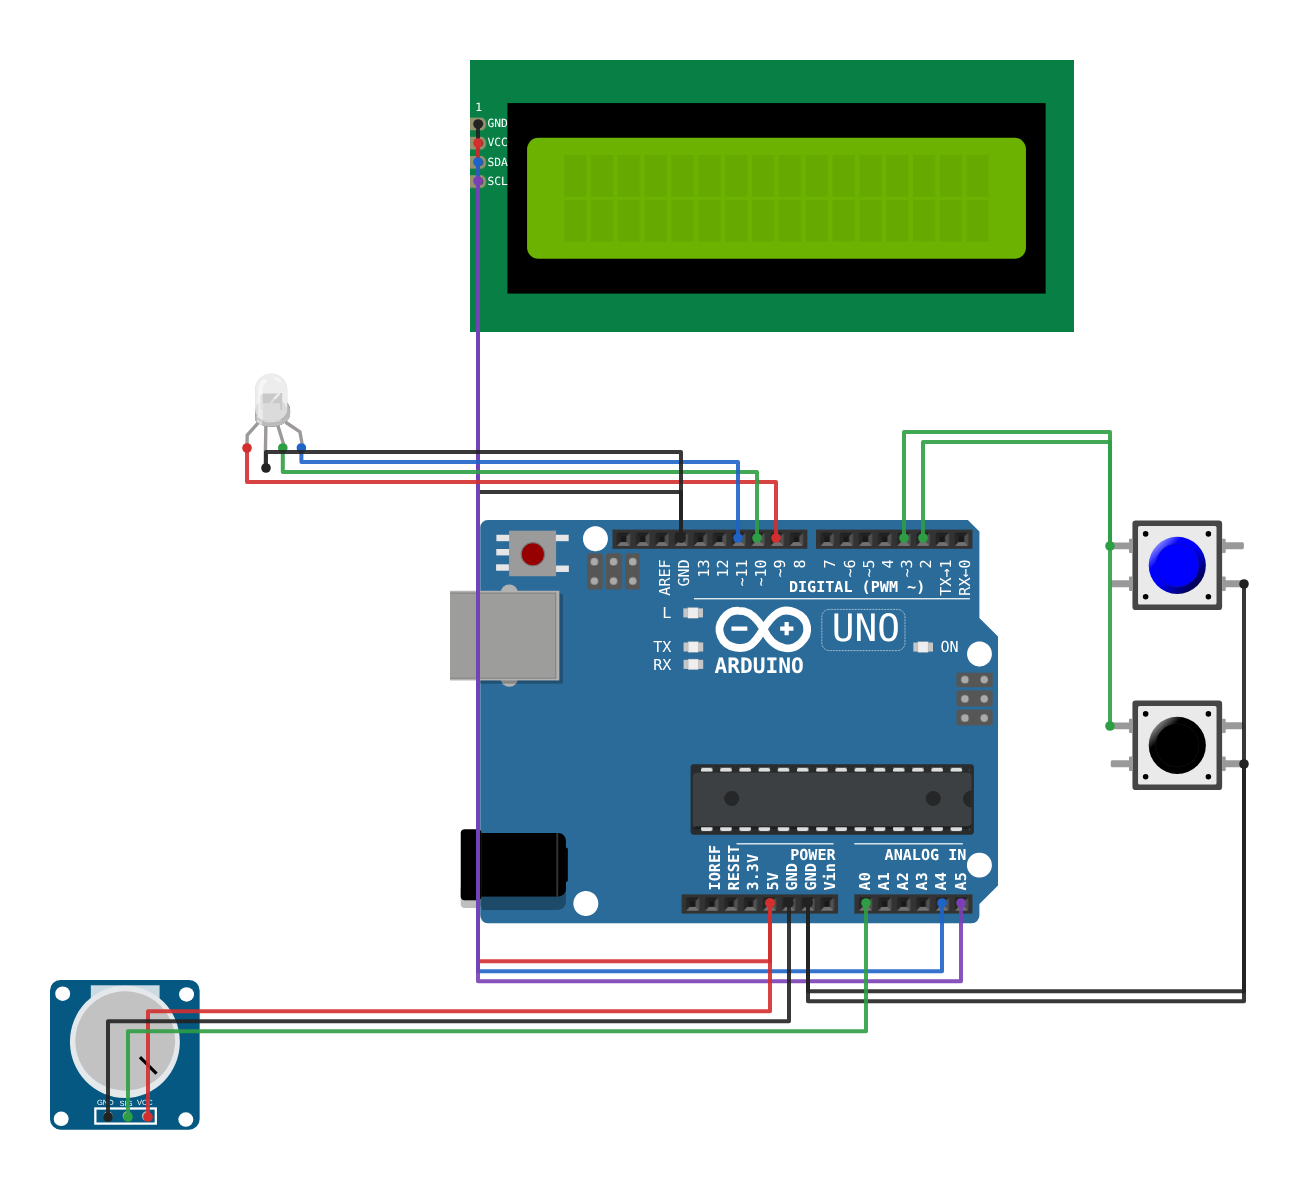
\includegraphics[width=.82\textwidth]{figuras/esquema-09.png}
\caption{Esquema do circuito da Automação 9, desenhado a partir do \texttt{diagram.json} com as peças do Wokwi}\label{fig:esq9}
\end{figure}

\paragraph{Funcionamento.} Cada cena é uma cor RGB: Leitura (branco neutro), Jantar (âmbar), Cinema (azul baixo, que não reflete na tela) e Festa. A troca interpola linearmente cada canal entre a cor de partida e a de destino ao longo de 1 s. Na cena Festa, terminada a transição, a cor percorre a roda de cores (matiz de 0 a 359$^\circ$) continuamente. O potenciômetro multiplica os três canais, o que muda o brilho sem alterar a tonalidade da cena. O algoritmo abaixo resume a decisão.

\begin{lstlisting}[style=algo]
se botão Cena: cena <- (cena + 1) mod 4; partida <- cor atual; destino <- cor da cena
se botão Desligar: cena <- apagada; destino <- preto
brilho <- potenciômetro / 4
t <- tempo desde o início da transição
se t < 1 s: cor <- partida + (destino - partida) * t / 1 s
senão se cena = Festa: a cada 20 ms, matiz <- matiz + 1; cor <- roda(matiz)
senão: cor <- destino
PWM de R, G e B <- canal * brilho / 255
\end{lstlisting}

\paragraph{Validação.} A Tabela~\ref{tab:val9} traz o roteiro de validação: cada estímulo aplicado e a resposta esperada, todos conferidos nos testes de lógica.

\begin{table}[ht]
\centering
\caption{Roteiro de validação da Automação 9}\label{tab:val9}
\footnotesize
\begin{tabularx}{\textwidth}{cXXc}
\toprule
Passo & Estímulo & Resposta & Situação \\
\midrule
1 & Ligar & LED apagado, LCD ``Cena: Apagada'' & OK \\
2 & Botão Cena & Transição suave até branco neutro (Leitura) & OK \\
3 & Botão Cena & Âmbar (Jantar) & OK \\
4 & Potenciômetro na metade & Brilho em 50\%, mesma cor & OK \\
5 & Botão Cena & Azul baixo (Cinema) & OK \\
6 & Botão Cena & Festa: cores girando & OK \\
7 & Botão Desligar & Apaga com esmaecimento & OK \\
8 & Botão Cena & Volta à cena Leitura & OK \\
\bottomrule
\end{tabularx}
\end{table}

\section{Resultados e discussão}\label{sec:result}

As nove automações compilaram sem avisos e passaram nas 93 verificações automáticas. As execuções do binário real no emulador AVR reproduziram as mesmas mensagens e decisões dos testes de lógica. A Tabela~\ref{tab:mem} mostra o uso de memória: a automação mais pesada, o portão por infravermelho, ocupa cerca de metade da flash por causa da biblioteca IRremote, e nenhuma passa de 46\% da SRAM.

\begin{table}[ht]
\centering
\caption{Uso de memória no ATmega328P}\label{tab:mem}
\footnotesize
\begin{tabularx}{\textwidth}{Xrrrr}
\toprule
Automação & Flash & \% de 32 KB & SRAM & \% de 2 KB \\
\midrule
Portão da garagem por controle remoto & 16546 B & 50,5\% & 928 B & 45,3\% \\
Alarme residencial com tempos de saída e entrada & 9838 B & 30,0\% & 727 B & 35,5\% \\
Luz do corredor com presença e vigília & 3488 B & 10,6\% & 282 B & 13,8\% \\
Cortina motorizada do quarto & 11718 B & 35,8\% & 612 B & 29,9\% \\
Irrigação do jardim por umidade do solo & 8404 B & 25,6\% & 634 B & 31,0\% \\
Ventilador de teto com velocidade automática & 6946 B & 21,2\% & 369 B & 18,0\% \\
Comedouro automático do pet com balança & 13436 B & 41,0\% & 878 B & 42,9\% \\
Campainha com modo ``não perturbe'' & 10070 B & 30,7\% & 753 B & 36,8\% \\
Cenas de iluminação da sala com LED RGB & 8372 B & 25,5\% & 592 B & 28,9\% \\
\bottomrule
\end{tabularx}
\end{table}

\subsection{Dificuldades encontradas}

\textbf{Sensores ausentes no simulador.} O Wokwi não oferece sensor de umidade do solo nem de chuva. A solução foi representar o primeiro por um potenciômetro, que gera a mesma faixa de tensão, e o segundo por uma chave. O código lê esses sinais exatamente como leria os sensores reais.

\textbf{Conflito de temporizadores.} A biblioteca IRremote e a função \texttt{tone()} usam o Timer2 do ATmega328P. Na Automação~1, o aviso sonoro foi substituído pelo pisca-alerta luminoso, e o servo ficou no Timer1.

\textbf{Botão único com duas funções.} No alarme, distinguir toque curto de toque longo exigiu acompanhar o instante em que o botão foi apertado e decidir só quando ele é solto ou quando o tempo passa de 2 s.

\textbf{Calibração da balança.} A célula de carga simulada entrega valores brutos; a escala de 0,42 foi obtida da faixa de 0 a 2100 para 5 kg.

\subsection{Integração na casa}

Embora independentes, as automações cobrem a rotina da casa. Ao chegar, o morador abre o portão pelo controle (1) e desarma o alarme (2). À noite, a cortina já fechou sozinha (4), a sala recebe a cena de jantar ou de cinema (9), o corredor guia quem levanta de madrugada (3) e o ventilador do quarto ajusta a velocidade conforme a noite esfria (6). Enquanto todos estão fora, o pet é alimentado (7), o jardim é regado só se precisar (5) e as visitas ficam registradas na campainha (8). Uma evolução natural é ligar essas placas a uma central: o alarme armado poderia fechar a cortina e apagar as luzes, e a campainha poderia avisar o celular.

\section{Considerações finais}\label{sec:final}

O trabalho mostrou que lógicas simples e bem modeladas (máquinas de estados, histerese e temporização sem bloqueio) bastam para automações residenciais úteis e previsíveis num microcontrolador de 8 bits.

\textbf{Limitações.} Os resultados vêm de simulação e de testes de lógica; sensores reais têm ruído e exigem calibração. Os sensores de solo e de chuva foram representados por componentes equivalentes. Não há comunicação entre as automações, e o alarme não tem senha, apenas o toque longo.

\textbf{Trabalhos futuros.} Migrar para o ESP32 e integrar as automações por Wi-Fi e MQTT a um painel no celular; acrescentar senha ou cartão RFID ao alarme; usar um relógio de tempo real para refeições e regas em horários fixos; e registrar o consumo de água da irrigação.

\bibliographystyle{sbc}
\bibliography{referencias}

\appendix

\section{Como executar as simulações}\label{ap:exec}

Repositório público do trabalho:

\begin{center}\url{https://github.com/USUARIO/REPOSITORIO}\end{center}

\noindent Cada automação está numa pasta na raiz do repositório (\texttt{01-portao-garagem} a \texttt{09-cenas-iluminacao}), com o programa (\texttt{sketch.ino}), o circuito (\texttt{diagram.json}), as bibliotecas (\texttt{libraries.txt}), o firmware compilado (\texttt{sketch.hex} e \texttt{sketch.elf}) e o arquivo \texttt{wokwi.toml}.

\paragraph{No navegador.} Em \url{https://wokwi.com}, crie um projeto \emph{Arduino Uno}, cole os três arquivos nas abas de mesmo nome (o \texttt{libraries.txt} é criado pela seta ao lado das abas) e inicie a simulação.

\paragraph{No Visual Studio Code.} Com a extensão \emph{Wokwi Simulator}, abra a pasta da automação e execute \emph{Wokwi: Start Simulator}; o firmware é carregado pelo \texttt{wokwi.toml}.

\paragraph{Dicas.} Teclas do controle remoto na Automação~1: PLAY alterna, + abre, $-$ fecha, POWER para. Na Automação~7, clique na célula de carga e aumente o peso enquanto a comporta está aberta. O monitor serial registra cada decisão dos programas.

\section{Código da Automação 1: Portão da garagem por controle remoto}

\noindent Pasta no repositório: \pasta{01-portao-garagem}. Bibliotecas: IRremote, Servo, LiquidCrystal I2C.

\begin{lstlisting}[language=C++]
// ---------------------------------------------------------------------------
// Casa Inteligente | 01 | Portão da garagem por controle remoto infravermelho
//
// O que faz: abre e fecha o portão (servo) pelo controle remoto, move o
// portão devagar, fecha sozinho depois de um tempo aberto e volta a abrir se
// a barreira de segurança detectar um obstáculo durante o fechamento.
//
// Entradas : receptor infravermelho (controle remoto) e botão que representa
//            a barreira de segurança (apertado = feixe interrompido).
// Saídas   : servo do portão, LED pisca-alerta e LCD 16x2 I2C.
//
// Teclas do controle do Wokwi:
//   PLAY  -> abre ou fecha (alterna)     +     -> abre
//   POWER -> parada de emergência         -     -> fecha
// ---------------------------------------------------------------------------
#include <IRremote.hpp>
#include <Servo.h>
#include <Wire.h>
#include <LiquidCrystal_I2C.h>

// pinos
const uint8_t pino_ir       = 2;
const uint8_t pino_barreira = 3;   // botão para o GND, pull-up interno
const uint8_t pino_servo    = 9;
const uint8_t pino_alerta   = 7;   // LED pisca-alerta

// códigos NEC das teclas do controle remoto do Wokwi
const uint8_t TECLA_POWER = 162;
const uint8_t TECLA_PLAY  = 168;
const uint8_t TECLA_MAIS  = 2;
const uint8_t TECLA_MENOS = 152;

// ajustes (tempos reduzidos para a simulação)
const int angulo_fechado = 0;
const int angulo_aberto  = 90;
const unsigned long passo_ms          = 40;     // 1 grau a cada 40 ms (~3,6 s de curso)
const unsigned long fechar_sozinho_ms = 15000;  // na prática, 2 minutos
const unsigned long pisca_ms          = 300;

enum class Portao : uint8_t { Fechado, Abrindo, Aberto, Fechando, Parado };

Servo motor;
LiquidCrystal_I2C lcd(0x27, 16, 2);

Portao estado = Portao::Fechado;
int angulo = angulo_fechado;
unsigned long ultimo_passo = 0;
unsigned long aberto_desde = 0;

const char *nome_estado(Portao e) {
  switch (e) {
    case Portao::Fechado:  return "FECHADO";
    case Portao::Abrindo:  return "ABRINDO";
    case Portao::Aberto:   return "ABERTO";
    case Portao::Fechando: return "FECHANDO";
    default:               return "PARADO";
  }
}

void mostrar() {
  char linha[17];
  snprintf(linha, sizeof linha, "Portao: %-8s", nome_estado(estado));
  lcd.setCursor(0, 0);
  lcd.print(linha);
  snprintf(linha, sizeof linha, "Abertura: %3d%% ", (angulo - angulo_fechado) * 100 / (angulo_aberto - angulo_fechado));
  lcd.setCursor(0, 1);
  lcd.print(linha);
}

void mudar(Portao novo) {
  if (novo == estado) return;
  estado = novo;
  if (novo == Portao::Aberto) aberto_desde = millis();
  Serial.print("[PORTAO] ");
  Serial.println(nome_estado(novo));
  mostrar();
}

// Decide o que fazer com cada tecla do controle, conforme o estado atual
void tratar_tecla(uint8_t tecla) {
  if (tecla == TECLA_POWER) {
    if (estado == Portao::Abrindo || estado == Portao::Fechando) mudar(Portao::Parado);
    return;
  }
  bool quer_abrir;
  if (tecla == TECLA_MAIS) quer_abrir = true;
  else if (tecla == TECLA_MENOS) quer_abrir = false;
  else if (tecla == TECLA_PLAY) quer_abrir = !(estado == Portao::Aberto || estado == Portao::Abrindo);
  else return;  // outras teclas não têm função

  if (quer_abrir && angulo < angulo_aberto) mudar(Portao::Abrindo);
  else if (!quer_abrir && angulo > angulo_fechado) mudar(Portao::Fechando);
}

void setup() {
  Serial.begin(9600);
  pinMode(pino_barreira, INPUT_PULLUP);
  pinMode(pino_alerta, OUTPUT);
  IrReceiver.begin(pino_ir);
  motor.attach(pino_servo);
  motor.write(angulo);
  lcd.init();
  lcd.backlight();
  mostrar();
}

void loop() {
  unsigned long agora = millis();

  // 1) controle remoto
  if (IrReceiver.decode()) {
    uint8_t tecla = IrReceiver.decodedIRData.command;
    IrReceiver.resume();
    Serial.print("[PORTAO] Tecla ");
    Serial.println(tecla);
    tratar_tecla(tecla);
  }

  // 2) segurança: obstáculo durante o fechamento faz o portão reabrir
  bool obstaculo = digitalRead(pino_barreira) == LOW;
  if (estado == Portao::Fechando && obstaculo) {
    Serial.println("[PORTAO] Obstaculo! Reabrindo");
    mudar(Portao::Abrindo);
  }

  // 3) fechamento automático (não fecha com obstáculo na frente)
  if (estado == Portao::Aberto && agora - aberto_desde >= fechar_sozinho_ms && !obstaculo) {
    mudar(Portao::Fechando);
  }

  // 4) movimento gradual do servo
  if ((estado == Portao::Abrindo || estado == Portao::Fechando) && agora - ultimo_passo >= passo_ms) {
    ultimo_passo = agora;
    angulo += (estado == Portao::Abrindo) ? 1 : -1;
    motor.write(angulo);
    if (angulo >= angulo_aberto) mudar(Portao::Aberto);
    else if (angulo <= angulo_fechado) mudar(Portao::Fechado);
    else if (angulo % 10 == 0) mostrar();
  }

  // 5) pisca-alerta enquanto o portão se move
  bool movendo = estado == Portao::Abrindo || estado == Portao::Fechando;
  digitalWrite(pino_alerta, movendo && (agora / pisca_ms) % 2 ? HIGH : LOW);
}
\end{lstlisting}

\section{Código da Automação 2: Alarme residencial com tempos de saída e entrada}

\noindent Pasta no repositório: \pasta{02-alarme-residencial}. Bibliotecas: LiquidCrystal I2C.

\begin{lstlisting}[language=C++]
// ---------------------------------------------------------------------------
// Casa Inteligente | 02 | Alarme residencial com tempo de saída e de entrada
//
// O que faz: protege a casa com um sensor de porta e um sensor de presença.
// Ao armar, o morador tem 10 s para sair. Se a porta abrir com o alarme
// armado, há 10 s para desarmar antes da sirene. Movimento dentro de casa com
// o alarme armado dispara na hora.
//
// Entradas : chave deslizante (sensor magnético da porta), sensor PIR e
//            botão de comando (toque curto arma; segurar 2 s desarma).
// Saídas   : buzzer (sirene), LEDs verde, amarelo e vermelho e LCD 16x2 I2C.
// ---------------------------------------------------------------------------
#include <Wire.h>
#include <LiquidCrystal_I2C.h>

const uint8_t pino_porta    = 2;   // HIGH = porta aberta
const uint8_t pino_pir      = 3;
const uint8_t pino_botao    = 4;   // para o GND, pull-up interno
const uint8_t pino_sirene   = 8;
const uint8_t led_verde     = 9;
const uint8_t led_amarelo   = 10;
const uint8_t led_vermelho  = 11;

const unsigned long tempo_saida_ms    = 10000;
const unsigned long tempo_entrada_ms  = 10000;
const unsigned long sirene_max_ms     = 30000;  // limite de tempo da sirene
const unsigned long segurar_ms        = 2000;   // toque longo para desarmar
const unsigned long filtro_botao_ms   = 50;

enum class Modo : uint8_t { Desarmado, Saida, Armado, Entrada, Disparado };

LiquidCrystal_I2C lcd(0x27, 16, 2);
Modo modo = Modo::Desarmado;
unsigned long inicio_modo = 0;
const char *motivo = "";
long ultimo_segundo = -1;   // última contagem mostrada no LCD
int fase_sirene = -1;       // tom atual da sirene (-1 = nenhum)

// --- leitura do botão: distingue toque curto e toque longo ---------------
struct LeituraBotao { bool curto; bool longo; };
bool botao_preso = false, longo_ja_avisado = false;
unsigned long botao_desde = 0, ultima_borda = 0;

LeituraBotao ler_botao() {
  LeituraBotao r = {false, false};
  bool apertado = digitalRead(pino_botao) == LOW;
  unsigned long agora = millis();
  if (apertado != botao_preso && agora - ultima_borda > filtro_botao_ms) {
    ultima_borda = agora;
    botao_preso = apertado;
    if (apertado) { botao_desde = agora; longo_ja_avisado = false; }
    else if (!longo_ja_avisado) r.curto = true;          // soltou antes de 2 s
  }
  if (botao_preso && !longo_ja_avisado && agora - botao_desde >= segurar_ms) {
    longo_ja_avisado = true;
    r.longo = true;                                       // segurou 2 s
  }
  return r;
}

void leds(bool verde, bool amarelo, bool vermelho) {
  digitalWrite(led_verde, verde);
  digitalWrite(led_amarelo, amarelo);
  digitalWrite(led_vermelho, vermelho);
}

void escrever(const char *l1, const char *l2) {
  char b[17];
  snprintf(b, sizeof b, "%-16s", l1); lcd.setCursor(0, 0); lcd.print(b);
  snprintf(b, sizeof b, "%-16s", l2); lcd.setCursor(0, 1); lcd.print(b);
}

void entrar(Modo novo) {
  modo = novo;
  inicio_modo = millis();
  ultimo_segundo = -1;
  fase_sirene = -1;
  noTone(pino_sirene);
  switch (novo) {
    case Modo::Desarmado: leds(true, false, false); escrever("Alarme", "DESARMADO"); Serial.println("[ALARME] Desarmado"); break;
    case Modo::Saida:     Serial.println("[ALARME] Armando: 10 s para sair"); break;
    case Modo::Armado:    leds(false, false, true); escrever("Alarme", "ARMADO"); Serial.println("[ALARME] Armado"); break;
    case Modo::Entrada:   Serial.println("[ALARME] Porta aberta: 10 s para desarmar"); break;
    case Modo::Disparado: escrever("DISPARADO!", motivo); Serial.print("[ALARME] DISPARO: "); Serial.println(motivo); break;
  }
}

// Mostra a contagem regressiva e bipa uma vez por segundo
void contagem(const char *titulo, unsigned long total, unsigned long decorrido, bool rapido) {
  long falta = (total - decorrido + 999) / 1000;
  if (falta != ultimo_segundo) {
    ultimo_segundo = falta;
    char l2[17];
    snprintf(l2, sizeof l2, "%ld s", falta);
    escrever(titulo, l2);
    tone(pino_sirene, rapido ? 2400 : 1600, rapido ? 250 : 80);
  }
  leds(false, (decorrido / 250) % 2, false);  // amarelo piscando
}

void setup() {
  Serial.begin(9600);
  pinMode(pino_porta, INPUT);
  pinMode(pino_pir, INPUT);
  pinMode(pino_botao, INPUT_PULLUP);
  pinMode(pino_sirene, OUTPUT);
  pinMode(led_verde, OUTPUT);
  pinMode(led_amarelo, OUTPUT);
  pinMode(led_vermelho, OUTPUT);
  lcd.init();
  lcd.backlight();
  entrar(Modo::Desarmado);
}

void loop() {
  unsigned long decorrido = millis() - inicio_modo;
  LeituraBotao botao = ler_botao();
  bool porta_aberta = digitalRead(pino_porta) == HIGH;
  bool movimento = digitalRead(pino_pir) == HIGH;

  // segurar 2 s desarma em qualquer situação
  if (botao.longo && modo != Modo::Desarmado) { entrar(Modo::Desarmado); return; }

  switch (modo) {
    case Modo::Desarmado:
      if (botao.curto) entrar(Modo::Saida);
      break;

    case Modo::Saida:
      if (decorrido >= tempo_saida_ms) {
        if (porta_aberta) { motivo = "Porta aberta"; entrar(Modo::Disparado); }  // saiu sem fechar
        else entrar(Modo::Armado);
      } else contagem("Saia e feche", tempo_saida_ms, decorrido, false);
      break;

    case Modo::Armado:
      if (movimento) { motivo = "Presenca interna"; entrar(Modo::Disparado); }
      else if (porta_aberta) entrar(Modo::Entrada);
      break;

    case Modo::Entrada:
      if (decorrido >= tempo_entrada_ms) { motivo = "Invasao porta"; entrar(Modo::Disparado); }
      else contagem("Desarme: segure", tempo_entrada_ms, decorrido, true);
      break;

    case Modo::Disparado: {
      int pisca = (decorrido / 300) % 2;
      leds(false, false, pisca);
      if (decorrido < sirene_max_ms) {
        if (pisca != fase_sirene) { fase_sirene = pisca; tone(pino_sirene, pisca ? 2200 : 1500); }  // sirene de dois tons
      } else if (fase_sirene != 2) {
        fase_sirene = 2;
        noTone(pino_sirene);   // sirene para, mas o LED segue avisando
      }
      break;
    }
  }
}
\end{lstlisting}

\section{Código da Automação 3: Luz do corredor com presença e vigília}

\noindent Pasta no repositório: \pasta{03-luz-corredor}. Bibliotecas: apenas o núcleo do Arduino.

\begin{lstlisting}[language=C++]
// ---------------------------------------------------------------------------
// Casa Inteligente | 03 | Luz do corredor com presença e luz de vigília
//
// O que faz: à noite, o corredor fica com uma luz fraca de vigília (10 %).
// Quando alguém passa, a luz acende em 100 % com subida suave, fica acesa
// enquanto houver movimento e apaga devagar 20 s depois do último movimento.
// De dia a lâmpada fica apagada, mesmo com movimento.
//
// Entradas : sensor de presença PIR e sensor de luminosidade (LDR).
// Saída    : lâmpada dimerizável (LED no pino PWM 9).
//
// Dia ou noite: leitura do LDR com histerese. Acima de 600 (cerca de 60 lux)
// passa a ser noite; abaixo de 520 (cerca de 100 lux) volta a ser dia.
// ---------------------------------------------------------------------------

const uint8_t pino_pir   = 2;
const uint8_t pino_ldr   = A0;
const uint8_t pino_lampada = 9;

const int limiar_noite = 600;
const int limiar_dia   = 520;
const uint8_t brilho_vigilia = 26;     // 10 % de 255
const uint8_t brilho_total   = 255;
const unsigned long manter_acesa_ms = 20000;  // na prática, 2 minutos
const unsigned long degrau_ms = 8;            // velocidade da rampa de brilho

bool noite = false;
unsigned long ultimo_movimento = 0;
bool ja_houve_movimento = false;
int brilho_atual = 0;
int brilho_alvo = 0;
unsigned long ultimo_degrau = 0;

// Atualiza "noite" só quando a leitura cruza um dos limiares (histerese)
void avaliar_luz_ambiente() {
  int leitura = analogRead(pino_ldr);   // mais escuro = valor maior
  bool antes = noite;
  if (!noite && leitura > limiar_noite) noite = true;
  else if (noite && leitura < limiar_dia) noite = false;
  if (noite != antes) {
    Serial.print("[CORREDOR] Agora e ");
    Serial.println(noite ? "NOITE" : "DIA");
  }
}

void setup() {
  Serial.begin(9600);
  pinMode(pino_pir, INPUT);
  pinMode(pino_lampada, OUTPUT);
  avaliar_luz_ambiente();
}

void loop() {
  unsigned long agora = millis();
  avaliar_luz_ambiente();

  if (digitalRead(pino_pir) == HIGH) {
    if (!ja_houve_movimento || agora - ultimo_movimento > 1000) Serial.println("[CORREDOR] Movimento");
    ultimo_movimento = agora;
    ja_houve_movimento = true;
  }
  bool alguem_passou = ja_houve_movimento && agora - ultimo_movimento < manter_acesa_ms;

  // Regra de decisão do brilho desejado
  int novo_alvo;
  if (!noite) novo_alvo = 0;                       // dia: apagada
  else if (alguem_passou) novo_alvo = brilho_total; // noite com presença
  else novo_alvo = brilho_vigilia;                  // noite sem presença
  if (novo_alvo != brilho_alvo) {
    brilho_alvo = novo_alvo;
    Serial.print("[CORREDOR] Brilho alvo: ");
    Serial.print(brilho_alvo * 100 / 255);
    Serial.println(" %");
  }

  // Rampa: aproxima o brilho do alvo um degrau por vez (acende e apaga suave)
  if (brilho_atual != brilho_alvo && agora - ultimo_degrau >= degrau_ms) {
    ultimo_degrau = agora;
    brilho_atual += (brilho_alvo > brilho_atual) ? 1 : -1;
    analogWrite(pino_lampada, brilho_atual);
  }
}
\end{lstlisting}

\section{Código da Automação 4: Cortina motorizada do quarto}

\noindent Pasta no repositório: \pasta{04-cortina-automatica}. Bibliotecas: Servo, LiquidCrystal I2C.

\begin{lstlisting}[language=C++]
// ---------------------------------------------------------------------------
// Casa Inteligente | 04 | Cortina motorizada do quarto
//
// O que faz: no modo automático, abre a cortina quando amanhece, fecha quando
// anoitece e fecha pela metade quando o sol bate direto na janela (para
// evitar calor e ofuscamento). No modo manual, os botões abrem e fecham em
// passos de 25 %.
//
// Entradas : sensor de luminosidade (LDR), chave deslizante Auto/Manual e
//            botões "Abrir" e "Fechar".
// Saídas   : servo da cortina (0 graus = fechada, 180 graus = aberta) e
//            LCD 16x2 I2C.
// ---------------------------------------------------------------------------
#include <Servo.h>
#include <Wire.h>
#include <LiquidCrystal_I2C.h>
#include <math.h>

const uint8_t pino_abrir  = 2;   // botões para o GND, pull-up interno
const uint8_t pino_fechar = 3;
const uint8_t pino_modo   = 4;   // chave: HIGH = automático, LOW = manual
const uint8_t pino_servo  = 6;
const uint8_t pino_ldr    = A0;

// faixas de luz (lux) usadas no modo automático
const float lux_amanheceu   = 50;     // abre acima disso
const float lux_anoiteceu   = 10;     // fecha abaixo disso
const float lux_sol_direto  = 20000;  // meia-cortina acima disso
const float lux_sol_passou  = 12000;  // volta a abrir abaixo disso

const unsigned long passo_servo_ms = 15;   // movimento suave
const unsigned long filtro_ms = 50;

Servo cortina;
LiquidCrystal_I2C lcd(0x27, 16, 2);

int posicao = 0;          // % de abertura atual
int alvo = 0;             // % de abertura desejada
int alvo_automatico = 0;  // última decisão do modo automático
float lux = 0;
unsigned long ultimo_passo = 0, ultima_tela = 0;

// Botões com filtro de repique: guarda o último estado estável de cada um
struct Botao { uint8_t pino; bool estavel; bool bruto; unsigned long mudou; };
Botao b_abrir = {pino_abrir, true, true, 0};
Botao b_fechar = {pino_fechar, true, true, 0};

bool apertou(Botao &b) {
  bool leitura = digitalRead(b.pino);
  if (leitura != b.bruto) { b.bruto = leitura; b.mudou = millis(); }
  if (millis() - b.mudou > filtro_ms && b.estavel != b.bruto) {
    b.estavel = b.bruto;
    return b.estavel == LOW;
  }
  return false;
}

// Curva do LDR do Wokwi: converte a leitura analógica em lux
float ler_lux() {
  int a = constrain(analogRead(pino_ldr), 1, 1022);
  float volts = a * 5.0 / 1024.0;
  float ohms = 2000.0 * volts / (1.0 - volts / 5.0);
  return pow(50e3 * pow(10, 0.7) / ohms, 1.0 / 0.7);
}

// Modo automático: máquina de três situações com histerese
int decidir_automatico(float l, int atual) {
  if (atual == 0) {                       // fechada (noite)
    return l > lux_amanheceu ? 100 : 0;
  }
  if (atual == 100) {                     // aberta (dia)
    if (l < lux_anoiteceu) return 0;
    if (l > lux_sol_direto) return 50;
    return 100;
  }
  // meia-cortina (sol direto)
  if (l < lux_anoiteceu) return 0;
  if (l < lux_sol_passou) return 100;
  return 50;
}

void setup() {
  Serial.begin(9600);
  pinMode(pino_abrir, INPUT_PULLUP);
  pinMode(pino_fechar, INPUT_PULLUP);
  pinMode(pino_modo, INPUT);
  cortina.attach(pino_servo);
  cortina.write(0);
  lcd.init();
  lcd.backlight();
}

void loop() {
  unsigned long agora = millis();
  bool automatico = digitalRead(pino_modo) == HIGH;
  lux = ler_lux();

  if (automatico) {
    int decisao = decidir_automatico(lux, alvo_automatico);
    if (decisao != alvo_automatico) {
      alvo_automatico = decisao;
      Serial.print("[CORTINA] Auto: ");
      Serial.print(decisao);
      Serial.print(" % (luz ");
      Serial.print((long)lux);
      Serial.println(" lux)");
    }
    alvo = alvo_automatico;
  }
  // Os botões funcionam só no manual; leitura feita sempre para não acumular toques
  bool abrir = apertou(b_abrir), fechar = apertou(b_fechar);
  if (!automatico) {
    if (abrir)  alvo = min(100, alvo + 25);
    if (fechar) alvo = max(0, alvo - 25);
    if (abrir || fechar) { Serial.print("[CORTINA] Manual: "); Serial.print(alvo); Serial.println(" %"); }
  }

  // Movimento suave: 1 % a cada 15 ms
  if (posicao != alvo && agora - ultimo_passo >= passo_servo_ms) {
    ultimo_passo = agora;
    posicao += (alvo > posicao) ? 1 : -1;
    cortina.write(map(posicao, 0, 100, 0, 180));
  }

  if (agora - ultima_tela >= 400) {
    ultima_tela = agora;
    char l1[17], l2[17];
    snprintf(l1, sizeof l1, "Cortina: %3d%%  ", posicao);
    snprintf(l2, sizeof l2, "%-6s %5ld lx ", automatico ? "AUTO" : "MANUAL", (long)(lux > 99999 ? 99999 : lux));
    lcd.setCursor(0, 0); lcd.print(l1);
    lcd.setCursor(0, 1); lcd.print(l2);
  }
}
\end{lstlisting}

\section{Código da Automação 5: Irrigação do jardim por umidade do solo}

\noindent Pasta no repositório: \pasta{05-irrigacao-jardim}. Bibliotecas: LiquidCrystal I2C.

\begin{lstlisting}[language=C++]
// ---------------------------------------------------------------------------
// Casa Inteligente | 05 | Irrigação do jardim por umidade do solo
//
// O que faz: rega o jardim só quando o solo está seco e não está chovendo.
// A rega é feita em ciclos curtos (rega, pausa para a água infiltrar,
// nova medição), o que evita encharcar o solo e desperdiçar água. Se o solo
// não melhora depois de 4 ciclos, o sistema para e avisa (possível vazamento
// ou sensor com defeito).
//
// Entradas : potenciômetro no lugar do sensor de umidade do solo (o Wokwi não
//            tem esse sensor), chave deslizante "chuva" e botão "Regar agora".
// Saídas   : relé da válvula solenoide (LED azul na carga) e LCD 16x2 I2C.
// ---------------------------------------------------------------------------
#include <Wire.h>
#include <LiquidCrystal_I2C.h>

const uint8_t pino_botao   = 2;   // para o GND, pull-up interno
const uint8_t pino_chuva   = 4;   // HIGH = chovendo
const uint8_t pino_valvula = 7;   // relé
const uint8_t pino_solo    = A0;

const int solo_seco    = 30;      // % abaixo do qual começa a regar
const int solo_umido   = 60;      // % em que para de regar
const unsigned long rega_ms     = 8000;    // na prática, 5 min por ciclo
const unsigned long pausa_ms    = 10000;   // na prática, 20 min de infiltração
const unsigned long manual_ms   = 5000;
const uint8_t ciclos_maximos    = 4;

enum Etapa : uint8_t { AGUARDANDO, REGANDO, INFILTRANDO, REGA_MANUAL, FALHA };
const char *const NOMES[] = {"Aguardando", "Regando", "Infiltrando", "Rega manual", "FALHA: verificar"};

LiquidCrystal_I2C lcd(0x27, 16, 2);
Etapa etapa = AGUARDANDO;
unsigned long inicio_etapa = 0;
uint8_t ciclos = 0;
int umidade = 0;
bool chovendo = false;

bool botao_anterior = HIGH;
unsigned long botao_mudou = 0;
bool botao_estavel = HIGH;

bool botao_apertado() {
  bool l = digitalRead(pino_botao);
  if (l != botao_anterior) { botao_anterior = l; botao_mudou = millis(); }
  if (millis() - botao_mudou > 50 && l != botao_estavel) { botao_estavel = l; return l == LOW; }
  return false;
}

void ir_para(Etapa nova) {
  etapa = nova;
  inicio_etapa = millis();
  digitalWrite(pino_valvula, (nova == REGANDO || nova == REGA_MANUAL) ? HIGH : LOW);
  Serial.print("[JARDIM] ");
  Serial.print(NOMES[nova]);
  Serial.print(" | solo ");
  Serial.print(umidade);
  Serial.print(" % | ciclo ");
  Serial.println(ciclos);
}

void setup() {
  Serial.begin(9600);
  pinMode(pino_botao, INPUT_PULLUP);
  pinMode(pino_chuva, INPUT);
  pinMode(pino_valvula, OUTPUT);
  lcd.init();
  lcd.backlight();
  ir_para(AGUARDANDO);
}

void loop() {
  unsigned long t = millis() - inicio_etapa;
  umidade = map(analogRead(pino_solo), 0, 1023, 0, 100);
  chovendo = digitalRead(pino_chuva) == HIGH;
  bool regar_agora = botao_apertado();

  // Chuva interrompe qualquer rega imediatamente
  if (chovendo && (etapa == REGANDO || etapa == INFILTRANDO || etapa == REGA_MANUAL)) {
    ciclos = 0;
    Serial.println("[JARDIM] Chuva detectada: rega cancelada");
    ir_para(AGUARDANDO);
  }

  switch (etapa) {
    case AGUARDANDO:
      if (regar_agora && !chovendo) ir_para(REGA_MANUAL);
      else if (!chovendo && umidade < solo_seco) { ciclos = 1; ir_para(REGANDO); }
      break;
    case REGANDO:
      if (umidade >= solo_umido) { ciclos = 0; ir_para(AGUARDANDO); }
      else if (t >= rega_ms) ir_para(INFILTRANDO);
      break;
    case INFILTRANDO:
      if (t < pausa_ms) break;
      if (umidade >= solo_umido) { ciclos = 0; ir_para(AGUARDANDO); }
      else if (ciclos >= ciclos_maximos) ir_para(FALHA);
      else { ciclos++; ir_para(REGANDO); }
      break;
    case REGA_MANUAL:
      if (t >= manual_ms) ir_para(AGUARDANDO);
      break;
    case FALHA:
      if (regar_agora) { ciclos = 0; ir_para(AGUARDANDO); }   // o botão reconhece a falha
      break;
  }

  static unsigned long tela = 0;
  if (millis() - tela >= 300) {
    tela = millis();
    char l1[17], l2[17];
    snprintf(l1, sizeof l1, "Solo:%3d%% %s", umidade, chovendo ? "CHUVA" : "     ");
    snprintf(l2, sizeof l2, "%-16s", NOMES[etapa]);
    lcd.setCursor(0, 0); lcd.print(l1);
    lcd.setCursor(0, 1); lcd.print(l2);
  }
}
\end{lstlisting}

\section{Código da Automação 6: Ventilador de teto com velocidade automática}

\noindent Pasta no repositório: \pasta{06-ventilador-teto}. Bibliotecas: DHT sensor library, Adafruit Unified Sensor.

\begin{lstlisting}[language=C++]
// ---------------------------------------------------------------------------
// Casa Inteligente | 06 | Ventilador de teto com velocidade automática
//
// O que faz: no modo automático, escolhe a velocidade do ventilador (0 a 3)
// pela sensação térmica, calculada a partir da temperatura e da umidade.
// O botão passa pelos modos Auto -> 1 -> 2 -> 3 -> Desligado -> Auto.
//
// Entradas : sensor DHT22 (temperatura e umidade) e botão de modo.
// Saídas   : display de 7 segmentos com a velocidade (ponto aceso = modo
//            automático) e o motor do ventilador, representado por um LED
//            com brilho proporcional à velocidade (PWM).
// ---------------------------------------------------------------------------
#include <DHT.h>

const uint8_t pino_dht   = 2;
const uint8_t pino_botao = 3;   // para o GND, pull-up interno
const uint8_t pino_motor = 9;   // PWM
// segmentos a, b, c, d, e, f, g e ponto do display (catodo comum)
const uint8_t segmentos[8] = {4, 5, 6, 7, 8, 10, 11, 12};

// padrões dos dígitos 0 a 3 (bit 0 = segmento a ... bit 6 = segmento g)
const uint8_t DIGITOS[4] = {0b0111111, 0b0000110, 0b1011011, 0b1001111};
const uint8_t PWM_POR_VELOCIDADE[4] = {0, 90, 170, 255};

// limites de sensação térmica (°C) para cada velocidade e histerese
const float limites[3] = {24.0, 26.5, 29.0};
const float histerese = 0.5;

enum Modo : uint8_t { AUTOMATICO, MANUAL_1, MANUAL_2, MANUAL_3, DESLIGADO };

DHT sensor(pino_dht, DHT22);
Modo modo = AUTOMATICO;
uint8_t velocidade = 0;
float sensacao = NAN;
unsigned long ultima_leitura = 0;
bool botao_antes = HIGH;
unsigned long botao_quando = 0;

// Sensação térmica simplificada: a umidade alta "esquenta" o ambiente
float calcular_sensacao(float t, float ur) {
  if (ur <= 60) return t;
  return t + (ur - 60) * 0.05;   // +0,5 °C a cada 10 % acima de 60 %
}

// Escolhe a velocidade com histerese: sobe ao passar do limite, desce só
// quando fica meio grau abaixo dele
uint8_t velocidade_automatica(float s, uint8_t atual) {
  uint8_t v = atual;
  while (v < 3 && s >= limites[v]) v++;
  while (v > 0 && s < limites[v - 1] - histerese) v--;
  return v;
}

void mostrar(uint8_t numero, bool ponto) {
  for (uint8_t i = 0; i < 7; i++) digitalWrite(segmentos[i], (DIGITOS[numero] >> i) & 1);
  digitalWrite(segmentos[7], ponto);
}

void aplicar(uint8_t v) {
  if (v != velocidade) {
    velocidade = v;
    Serial.print("[VENTILADOR] Velocidade ");
    Serial.println(v);
  }
  analogWrite(pino_motor, PWM_POR_VELOCIDADE[velocidade]);
  mostrar(velocidade, modo == AUTOMATICO);
}

void setup() {
  Serial.begin(9600);
  pinMode(pino_botao, INPUT_PULLUP);
  pinMode(pino_motor, OUTPUT);
  for (uint8_t p : segmentos) pinMode(p, OUTPUT);
  sensor.begin();
  aplicar(0);
  ultima_leitura = millis() - 2000;   // primeira leitura logo no início
}

void loop() {
  unsigned long agora = millis();

  // Botão: cada toque avança um modo
  bool b = digitalRead(pino_botao);
  if (b != botao_antes && agora - botao_quando > 50) {
    botao_quando = agora;
    botao_antes = b;
    if (b == LOW) {
      modo = (Modo)((modo + 1) % 5);
      Serial.print("[VENTILADOR] Modo ");
      Serial.println(modo == AUTOMATICO ? "automatico" : modo == DESLIGADO ? "desligado" : "manual");
    }
  }

  // Leitura do sensor a cada 2 s (limite do DHT22)
  if (agora - ultima_leitura >= 2000) {
    ultima_leitura = agora;
    float t = sensor.readTemperature(), ur = sensor.readHumidity();
    if (!isnan(t) && !isnan(ur)) {
      sensacao = calcular_sensacao(t, ur);
      Serial.print("[VENTILADOR] T=");
      Serial.print(t, 1);
      Serial.print(" C UR=");
      Serial.print(ur, 0);
      Serial.print(" % sensacao=");
      Serial.println(sensacao, 1);
    }
  }

  // Decisão da velocidade conforme o modo
  uint8_t v;
  switch (modo) {
    case AUTOMATICO: v = isnan(sensacao) ? 1 : velocidade_automatica(sensacao, velocidade); break;  // sem leitura: velocidade 1 por segurança
    case MANUAL_1:   v = 1; break;
    case MANUAL_2:   v = 2; break;
    case MANUAL_3:   v = 3; break;
    default:         v = 0; break;
  }
  aplicar(v);
}
\end{lstlisting}

\section{Código da Automação 7: Comedouro automático do pet com balança}

\noindent Pasta no repositório: \pasta{07-comedouro-pet}. Bibliotecas: HX711, Servo, LiquidCrystal I2C.

\begin{lstlisting}[language=C++]
// ---------------------------------------------------------------------------
// Casa Inteligente | 07 | Comedouro automático do pet com balança
//
// O que faz: nos horários programados (ou pelo botão), libera ração até o
// pote atingir a porção de 100 g. Se o pote ainda tem ração suficiente, não
// serve de novo (evita excesso). Se a ração não cai em 8 s, o reservatório
// provavelmente acabou: o sistema fecha a comporta e avisa.
//
// Entradas : célula de carga com módulo HX711 (peso do pote) e botão
//            "Servir agora".
// Saídas   : servo da comporta, buzzer, LED "reservatório vazio" e LCD 16x2.
//
// No Wokwi: durante a liberação, aumente o peso da célula de carga (clique
// nela) para simular a ração caindo no pote.
// ---------------------------------------------------------------------------
#include <HX711.h>
#include <Servo.h>
#include <Wire.h>
#include <LiquidCrystal_I2C.h>

const uint8_t pino_hx_dt  = A1;
const uint8_t pino_hx_sck = A0;
const uint8_t pino_botao  = 2;   // para o GND, pull-up interno
const uint8_t pino_servo  = 6;
const uint8_t pino_buzzer = 8;
const uint8_t pino_led_vazio = 9;

const float escala = 0.42;                     // célula de 5 kg do Wokwi: leitura bruta 0-2100 = 0-5000 g
const float porcao_g = 100;                    // porção por refeição
const float minimo_para_pular_g = 60;          // com 60 g ou mais no pote, não serve
const unsigned long intervalo_refeicao_ms = 30000;  // na prática, a cada 8 horas
const unsigned long tempo_maximo_ms = 8000;    // sem atingir a porção: reservatório vazio
const int comporta_fechada = 0, comporta_aberta = 70;

enum Situacao : uint8_t { ESPERANDO, SERVINDO, VAZIO };

HX711 balanca;
Servo comporta;
LiquidCrystal_I2C lcd(0x27, 16, 2);

Situacao situacao = ESPERANDO;
float peso = 0;
unsigned long proxima_refeicao = 0;
unsigned long inicio_servico = 0;
unsigned long ultimo_bipe = 0;
uint8_t refeicoes_servidas = 0;
bool botao_era = HIGH;
unsigned long botao_t = 0;

bool pediu_agora() {
  bool b = digitalRead(pino_botao);
  bool borda = false;
  if (b != botao_era && millis() - botao_t > 50) { botao_t = millis(); botao_era = b; borda = (b == LOW); }
  return borda;
}

void tela() {
  char l1[17], l2[17];
  snprintf(l1, sizeof l1, "Pote: %4d g    ", (int)peso);
  if (situacao == SERVINDO) snprintf(l2, sizeof l2, "Servindo...     ");
  else if (situacao == VAZIO) snprintf(l2, sizeof l2, "RACAO ACABOU!   ");
  else {
    long falta = ((long)proxima_refeicao - (long)millis()) / 1000;
    snprintf(l2, sizeof l2, "Prox. em %3lds  ", falta < 0 ? 0L : (falta > 999 ? 999L : falta));
  }
  lcd.setCursor(0, 0); lcd.print(l1);
  lcd.setCursor(0, 1); lcd.print(l2);
}

// Início de uma refeição: decide se precisa servir
void refeicao(const char *origem) {
  proxima_refeicao = millis() + intervalo_refeicao_ms;
  Serial.print("[COMEDOURO] Refeicao (");
  Serial.print(origem);
  Serial.print("), pote com ");
  Serial.print((int)peso);
  Serial.println(" g");
  if (peso >= minimo_para_pular_g) {
    Serial.println("[COMEDOURO] Ainda ha racao no pote: nao serve");
    tone(pino_buzzer, 600, 120);
    return;
  }
  situacao = SERVINDO;
  inicio_servico = millis();
  comporta.write(comporta_aberta);
}

void terminar(Situacao nova) {
  comporta.write(comporta_fechada);
  situacao = nova;
  if (nova == ESPERANDO) {
    refeicoes_servidas++;
    tone(pino_buzzer, 1800, 150);   // "a comida está servida"
    Serial.print("[COMEDOURO] Porcao servida. Total hoje: ");
    Serial.println(refeicoes_servidas);
  } else {
    Serial.println("[COMEDOURO] Racao nao caiu: reservatorio vazio");
  }
}

void setup() {
  Serial.begin(9600);
  pinMode(pino_botao, INPUT_PULLUP);
  pinMode(pino_buzzer, OUTPUT);
  pinMode(pino_led_vazio, OUTPUT);
  balanca.begin(pino_hx_dt, pino_hx_sck);
  balanca.set_scale(escala);
  comporta.attach(pino_servo);
  comporta.write(comporta_fechada);
  lcd.init();
  lcd.backlight();
  proxima_refeicao = millis() + intervalo_refeicao_ms;
}

void loop() {
  unsigned long agora = millis();
  if (balanca.is_ready()) peso = max(0.0f, balanca.get_units(1));
  bool pedido = pediu_agora();

  switch (situacao) {
    case ESPERANDO:
      if (pedido) refeicao("botao");
      else if ((long)(agora - proxima_refeicao) >= 0) refeicao("horario");
      break;
    case SERVINDO:
      if (peso >= porcao_g) terminar(ESPERANDO);
      else if (agora - inicio_servico >= tempo_maximo_ms) terminar(VAZIO);
      break;
    case VAZIO:
      // Bipe a cada 3 s até alguém reabastecer e apertar o botão
      if (agora - ultimo_bipe >= 3000) { ultimo_bipe = agora; tone(pino_buzzer, 900, 300); }
      if (pedido) {
        situacao = ESPERANDO;
        Serial.println("[COMEDOURO] Reabastecido: tentando servir de novo");
        refeicao("reabastecido");
      }
      break;
  }
  digitalWrite(pino_led_vazio, situacao == VAZIO ? HIGH : LOW);

  static unsigned long ultima_tela = 0;
  if (agora - ultima_tela >= 300) { ultima_tela = agora; tela(); }
}
\end{lstlisting}

\section{Código da Automação 8: Campainha com modo ``não perturbe''}

\noindent Pasta no repositório: \pasta{08-campainha}. Bibliotecas: LiquidCrystal I2C.

\begin{lstlisting}[language=C++]
// ---------------------------------------------------------------------------
// Casa Inteligente | 08 | Campainha com modo "não perturbe"
//
// O que faz: ao apertar a campainha, toca uma melodia curta e registra a
// visita. Toques repetidos em menos de 4 s contam como a mesma visita (a
// pessoa insistindo). Com o modo "não perturbe" ligado, a campainha fica
// muda: só o LED pisca e a visita fica guardada como perdida. Ao desligar
// esse modo, o display mostra quantas visitas foram perdidas.
//
// Entradas : botão da campainha e chave deslizante "Não perturbe".
// Saídas   : buzzer (melodia), LED de aviso e LCD 16x2 I2C.
// ---------------------------------------------------------------------------
#include <Wire.h>
#include <LiquidCrystal_I2C.h>

const uint8_t pino_campainha = 2;   // para o GND, pull-up interno
const uint8_t pino_silencio  = 4;   // chave: HIGH = não perturbe ligado
const uint8_t pino_buzzer    = 8;
const uint8_t pino_led       = 9;

const unsigned long mesma_visita_ms = 4000;
const unsigned long led_aviso_ms    = 5000;

// melodia "ding-dong-ding" (frequência em Hz, duração em ms)
struct Nota { unsigned int hz; unsigned int ms; };
const Nota MELODIA[] = {{1319, 220}, {1047, 220}, {1568, 400}};
const uint8_t TOTAL_NOTAS = sizeof(MELODIA) / sizeof(MELODIA[0]);

LiquidCrystal_I2C lcd(0x27, 16, 2);

unsigned int visitas = 0, perdidas = 0;
unsigned long ultima_visita = 0;
bool ja_teve_visita = false;
int nota_atual = -1;                 // -1 = melodia parada
unsigned long inicio_nota = 0;
unsigned long led_ate = 0;
bool silencio_antes = false;
bool botao_antes = HIGH;
unsigned long botao_t = 0;

void escrever(const char *l1, const char *l2) {
  char b[17];
  snprintf(b, sizeof b, "%-16s", l1); lcd.setCursor(0, 0); lcd.print(b);
  snprintf(b, sizeof b, "%-16s", l2); lcd.setCursor(0, 1); lcd.print(b);
}

void painel_normal() {
  char l1[17], l2[17];
  snprintf(l1, sizeof l1, "Visitas: %u", visitas);
  snprintf(l2, sizeof l2, "%s", digitalRead(pino_silencio) ? "Nao perturbe" : "Campainha ativa");
  escrever(l1, l2);
}

// Toca a melodia sem travar o programa: uma nota por vez, pelo relógio
void atualizar_melodia() {
  if (nota_atual < 0) return;
  if (millis() - inicio_nota < MELODIA[nota_atual].ms) return;
  nota_atual++;
  if (nota_atual >= TOTAL_NOTAS) { nota_atual = -1; noTone(pino_buzzer); return; }
  inicio_nota = millis();
  tone(pino_buzzer, MELODIA[nota_atual].hz);
}

void tocar() {
  nota_atual = 0;
  inicio_nota = millis();
  tone(pino_buzzer, MELODIA[0].hz);
}

void registrar_toque(bool silencio) {
  unsigned long agora = millis();
  bool insistencia = ja_teve_visita && agora - ultima_visita < mesma_visita_ms;
  ultima_visita = agora;
  ja_teve_visita = true;
  led_ate = agora + led_aviso_ms;
  if (insistencia) {
    Serial.println("[CAMPAINHA] Toque repetido: mesma visita");
    return;                                      // não toca de novo nem conta
  }
  visitas++;
  if (silencio) {
    perdidas++;
    Serial.println("[CAMPAINHA] Visita em modo nao perturbe (so LED)");
    escrever("Visita (mudo)", "");
  } else {
    Serial.println("[CAMPAINHA] Ding-dong!");
    tocar();
    escrever("Ding-dong!", "Alguem na porta");
  }
}

void setup() {
  Serial.begin(9600);
  pinMode(pino_campainha, INPUT_PULLUP);
  pinMode(pino_silencio, INPUT);
  pinMode(pino_buzzer, OUTPUT);
  pinMode(pino_led, OUTPUT);
  lcd.init();
  lcd.backlight();
  silencio_antes = digitalRead(pino_silencio);
  painel_normal();
}

void loop() {
  unsigned long agora = millis();
  bool silencio = digitalRead(pino_silencio) == HIGH;

  bool b = digitalRead(pino_campainha);
  if (b != botao_antes && agora - botao_t > 50) {
    botao_t = agora;
    botao_antes = b;
    if (b == LOW) registrar_toque(silencio);
  }

  // Ao sair do "não perturbe", avisa as visitas perdidas
  if (silencio != silencio_antes) {
    silencio_antes = silencio;
    if (!silencio && perdidas > 0) {
      char l2[17];
      snprintf(l2, sizeof l2, "%u perdida(s)", perdidas);
      escrever("Enquanto mudo:", l2);
      Serial.print("[CAMPAINHA] Visitas perdidas: ");
      Serial.println(perdidas);
      perdidas = 0;
      led_ate = agora + led_aviso_ms;
    } else {
      painel_normal();
    }
  }

  atualizar_melodia();

  // LED pisca enquanto houver aviso pendente
  bool aviso = (long)(led_ate - agora) > 0;
  digitalWrite(pino_led, aviso && (agora / 250) % 2 ? HIGH : LOW);
  static bool aviso_antes = false;
  if (aviso_antes && !aviso) painel_normal();    // aviso terminou: volta ao painel
  aviso_antes = aviso;
}
\end{lstlisting}

\section{Código da Automação 9: Cenas de iluminação da sala com LED RGB}

\noindent Pasta no repositório: \pasta{09-cenas-iluminacao}. Bibliotecas: LiquidCrystal I2C.

\begin{lstlisting}[language=C++]
// ---------------------------------------------------------------------------
// Casa Inteligente | 09 | Cenas de iluminação da sala com LED RGB
//
// O que faz: um botão percorre cenas prontas (Leitura, Jantar, Cinema e
// Festa), com transição suave de 1 s entre as cores. O potenciômetro regula
// o brilho geral. Na cena Festa, as cores giram sozinhas. O outro botão
// apaga a sala com esmaecimento.
//
// Entradas : botão "Cena", botão "Desligar" e potenciômetro de brilho.
// Saídas   : LED RGB (fita de LED da sanca, catodo comum) e LCD 16x2 I2C.
// ---------------------------------------------------------------------------
#include <Wire.h>
#include <LiquidCrystal_I2C.h>

const uint8_t pino_cena     = 2;   // botões para o GND, pull-up interno
const uint8_t pino_desligar = 3;
const uint8_t pino_brilho   = A0;
const uint8_t pino_r = 9, pino_g = 10, pino_b = 11;   // PWM

struct Cor { uint8_t r, g, b; };
struct Cena { const char *nome; Cor cor; };

const Cena CENAS[] = {
  {"Leitura", {255, 244, 229}},   // branco neutro, luz para ler
  {"Jantar",  {255, 147, 41}},    // âmbar quente
  {"Cinema",  {20, 30, 120}},     // azul baixo, sem reflexo na tela
  {"Festa",   {255, 0, 0}},       // ponto de partida do ciclo de cores
};
const uint8_t TOTAL_CENAS = sizeof(CENAS) / sizeof(CENAS[0]);
const uint8_t CENA_FESTA = 3;
const unsigned long transicao_ms = 1000;

LiquidCrystal_I2C lcd(0x27, 16, 2);

int cena = -1;                  // -1 = sala apagada
Cor cor_de = {0, 0, 0}, cor_para = {0, 0, 0}, cor_agora = {0, 0, 0};
unsigned long inicio_transicao = 0;
uint8_t brilho = 255;
uint16_t matiz = 0;             // usado no ciclo da cena Festa (0 a 359 graus)

struct Botao { uint8_t pino; bool antes; unsigned long t; };
Botao b_cena = {pino_cena, HIGH, 0}, b_desligar = {pino_desligar, HIGH, 0};

bool apertou(Botao &b) {
  bool l = digitalRead(b.pino);
  if (l != b.antes && millis() - b.t > 50) { b.t = millis(); b.antes = l; return l == LOW; }
  return false;
}

// Converte matiz (0-359) em cor RGB com saturação e valor máximos
Cor roda_de_cores(uint16_t h) {
  uint8_t setor = h / 60, f = (h % 60) * 255 / 60;
  switch (setor) {
    case 0:  return {255, f, 0};
    case 1:  return {(uint8_t)(255 - f), 255, 0};
    case 2:  return {0, 255, f};
    case 3:  return {0, (uint8_t)(255 - f), 255};
    case 4:  return {f, 0, 255};
    default: return {255, 0, (uint8_t)(255 - f)};
  }
}

uint8_t misturar(uint8_t a, uint8_t b, unsigned long t) {
  return a + ((long)b - a) * (long)t / (long)transicao_ms;
}

void iniciar_transicao(Cor destino) {
  cor_de = cor_agora;
  cor_para = destino;
  inicio_transicao = millis();
}

void atualizar_lcd() {
  char l1[17], l2[17];
  snprintf(l1, sizeof l1, "Cena: %-10s", cena < 0 ? "Apagada" : CENAS[cena].nome);
  snprintf(l2, sizeof l2, "Brilho: %3d%%    ", brilho * 100 / 255);
  lcd.setCursor(0, 0); lcd.print(l1);
  lcd.setCursor(0, 1); lcd.print(l2);
}

void setup() {
  Serial.begin(9600);
  pinMode(pino_cena, INPUT_PULLUP);
  pinMode(pino_desligar, INPUT_PULLUP);
  pinMode(pino_r, OUTPUT);
  pinMode(pino_g, OUTPUT);
  pinMode(pino_b, OUTPUT);
  lcd.init();
  lcd.backlight();
  atualizar_lcd();
}

void loop() {
  unsigned long agora = millis();

  if (apertou(b_cena)) {
    cena = (cena + 1) % TOTAL_CENAS;
    matiz = 0;
    iniciar_transicao(CENAS[cena].cor);
    Serial.print("[SALA] Cena: ");
    Serial.println(CENAS[cena].nome);
    atualizar_lcd();
  }
  if (apertou(b_desligar) && cena >= 0) {
    cena = -1;
    iniciar_transicao({0, 0, 0});
    Serial.println("[SALA] Apagando");
    atualizar_lcd();
  }

  // Brilho geral pelo potenciômetro (só atualiza o LCD quando muda bastante)
  uint8_t novo_brilho = analogRead(pino_brilho) / 4;
  if (abs((int)novo_brilho - (int)brilho) > 3) { brilho = novo_brilho; atualizar_lcd(); }

  // Transição linear entre a cor de partida e a de destino
  unsigned long t = agora - inicio_transicao;
  if (t >= transicao_ms) {
    cor_agora = cor_para;
    // Na cena Festa, terminada a transição, a cor gira continuamente
    if (cena == CENA_FESTA) {
      static unsigned long ultimo_giro = 0;
      if (agora - ultimo_giro >= 20) { ultimo_giro = agora; matiz = (matiz + 1) % 360; cor_agora = cor_para = roda_de_cores(matiz); }
    }
  } else {
    cor_agora = {misturar(cor_de.r, cor_para.r, t), misturar(cor_de.g, cor_para.g, t), misturar(cor_de.b, cor_para.b, t)};
  }

  analogWrite(pino_r, cor_agora.r * brilho / 255);
  analogWrite(pino_g, cor_agora.g * brilho / 255);
  analogWrite(pino_b, cor_agora.b * brilho / 255);
}
\end{lstlisting}

\end{document}
